\documentclass[pdftex,10pt,b5paper,twoside,openright]{report}
\PassOptionsToPackage{hyphens}{url}\usepackage[pdfborder={0 0 0}, breaklinks = true]{hyperref}
\usepackage[nameinlink, noabbrev]{cleveref}
\usepackage[lmargin=25mm,rmargin=25mm,tmargin=27mm,bmargin=30mm]{geometry}
\usepackage[utf8]{inputenc}
\usepackage[english]{babel}
\usepackage{graphicx}
\usepackage{pdfpages}
\usepackage{attachfile}
\usepackage{float}
\usepackage[acronym, nonumberlist, toc, nogroupskip]{glossaries}
\usepackage{listing}
\usepackage{listings}
\usepackage{mdwlist}
\usepackage{lstcustom}
\definecolor{shadecolor}{rgb}{1, 0.8, 0.3}
\usepackage{framed, color}
\usepackage{subcaption}
\usepackage{microtype}
\usepackage[font={small}, labelfont=bf]{caption}
\usepackage{emptypage}

% the file that contains our syntax highlighting configuration for the lst listings. 
% Color definitions for syntax highlighting

% Python
\definecolor{pythoncomment}{RGB}{0,0,255} 
\definecolor{pythonstring}{RGB}{255,0,255} 
\definecolor{pythonkeyword}{RGB}{165,42,42}

% Java
\definecolor{javacomment}{RGB}{0,0,255} 
\definecolor{javastring}{RGB}{255,0,255} 
\definecolor{javakeyword}{RGB}{165,42,42} 

% Bash
\definecolor{bashcomment}{RGB}{0,0,255}
\definecolor{bashstring}{RGB}{255,0,255}
\definecolor{bashkeyword}{RGB}{165,42,42}

% C++
\definecolor{c++comment}{RGB}{0,0,255}
\definecolor{c++string}{RGB}{255,0,255}
\definecolor{c++keyword}{RGB}{46,139,87}


% Code listing styles
\lstdefinestyle{java}
    {keywordstyle=\color{javakeyword}\bfseries,
    commentstyle=\color{javacomment},
    stringstyle=\color{javastring},
    morecomment=[s][\color{javacomment}]{/**}{*/}
}

\lstdefinestyle{python}
  {keywordstyle=\color{pythonkeyword},      
  commentstyle=\color{pythoncomment},      
  stringstyle=\color{pythonstring}  
}

\lstdefinestyle{bash}
    {keywordstyle=\color{bashkeyword},
    commentstyle=\color{bashcomment},
    stringstyle=\color{bashstring}
}

\lstdefinestyle{c++}
    {keywordstyle=\color{c++keyword},
    commentstyle=\color{c++comment},
    stringstyle=\color{c++string}
}

\lstdefinelanguage{xml}
{
  morestring=[b]",
  morestring=[s]{>}{<},
  morecomment=[s]{<?}{?>},
  stringstyle=\color{black},
  identifierstyle=\color{darkblue},
  keywordstyle=\color{cyan},
  morekeywords={xmlns,version, type, return, ns2, S, Envelope, Body, config, 
                RoutingInfo, RoutingInfos, services, service, name, destIP, 
                lastTR, bandwidth, client, role}% list your attributes here
}


\newglossarystyle{superbold}{%
  \renewenvironment{theglossary}%
    {\tablehead{}\tabletail{}%
     \begin{supertabular}{lp{\glsdescwidth}}}%
    {\end{supertabular}}%
  \renewcommand*{\glossaryheader}{}%
  \renewcommand*{\glsgroupheading}[1]{}%
  \renewcommand{\glossentry}[2]{%
    \glsentryitem{##1}\glstarget{##1}{\textbf{\glossentryname{##1}}} &
    \glossentrydesc{##1}\glspostdescription\space ##2\tabularnewline
  }%
  \renewcommand{\subglossentry}[3]{%
     &
     \glssubentryitem{##2}%
     \glstarget{##2}{\strut}\glossentrydesc{##2}\glspostdescription\space
     ##3\tabularnewline
  }%
  \renewcommand*{\glsgroupskip}{%
    \ifglsnogroupskip\else & \tabularnewline\fi}%
}

% the file containing all the words in our glossary. 
%A
\newglossaryentry{agile}{name={Agile methods}, description={
A group of software development methodologies based on iterative and incremental development.\\
\url{http://en.wikipedia.org/wiki/Agile_software_development}}}

\newglossaryentry{synapse}{name={Apache Synapse}, description={
A lightweight and high-performance Enterprise Service Bus.\\
\url{http://synapse.apache.org/}}}
%B
\newglossaryentry{bandwidth}{name={bandwidth}, description={
Available or consumed data communication resources.\\
\url{https://secure.wikimedia.org/wikipedia/en/wiki/Bandwidth_(computing)}}}

\newglossaryentry{breakpoint}{name={breakpoint}, description={
A source code marker telling the debugger to halt program execution at a certain point.}}

\newglossaryentry{broker}{name={Broker} , description={
Our middleware layer works as a QoS broker for services and clients.
Broker as referred to by the report given to us from FFI: a centralized ‘server’ of sorts which gathered Bandwidth data from tactical routers.}}

%C
\newglossaryentry{cli}{name={CLI}, description={
Command Line Interface, a text-based interface for interacting with programs via a terminal.}}

\newglossaryentry{codecanvas}{name={Code Canvas}, description={
A visualization-tool for Microsoft visual studio, showing code, diagrams and documents on a large layered canvas.\\
\url{http://research.microsoft.com/en-us/projects/codecanvas/}}}

\newglossaryentry{contourdiagram}{name={contour diagram}, description={
An enhanced object diagram, showing objects, their variables and their relations to other objects.\\
\cite{Jayaraman1996, Streib2010}}}%TODO:refer to paper

\newglossaryentry{cots}{name={COTS} , description={
Commercially available Off-The-Shelf often used to talk about services which the customer wants to use server side.\\ \url{https://secure.wikimedia.org/wikipedia/en/wiki/Commercial_off-the-shelf}}}

\newglossaryentry{credentials}{name={credentials} , description={
User-supplied credentials in the form of a username, password, role triplet.}}

%D
\newglossaryentry{debugVisualizationPlugin}{name={Debug Visualization Plugin}, description={
An Eclipse plugin that provides a graphical view of variables during debugging.\\
\url{https://code.google.com/a/eclipselabs.org/p/debugvisualisation/}}}

\newglossaryentry{diffserv}{name={DiffServ} , description={
Differentiated services, a field in the IPv4 header.\\
\url{http://www.networksorcery.com/enp/rfc/rfc2474.txt}}}

%E
\newglossaryentry{esb}{name={ESB} , description={
A software architecture model used for designing and the interaction and communication between mutually interacting software applications.\\ \url{http://en.wikipedia.org/wiki/Enterprise_service_bus}}}

\newglossaryentry{executiontrace}{name={execution trace} ,description={
A log of all changes to the state of a program throughout its execution.}}

%G
\newglossaryentry{gantt}{name={Gantt Chart}, description={
A type of bar chart that illustrates a project schedule.\\
\url{http://en.wikipedia.org/wiki/Gantt}}}

\newglossaryentry{gdb}{name={GDB}, description={
GNU debugger. A multiplatform, multilanguage CLI-debugger with tracing.\\
\url{http://www.sourceware.org/gdb/}}}

\newglossaryentry{git}{name={Git} , description={
A free and open source, distributed version control system.\\
\url{http://www.git-scm.com}}}

\newglossaryentry{github}{name={GitHub} , description={
A web-based hosting service for software development projects that use the Git version control system.\\
\url{http://www.github.com}}}

\newglossaryentry{glassfish}{name={GlassFish} , description={
An application server written in Java.\\
\url{http://glassfish.java.net/}}}

%H
\newglossaryentry{http}{name={HTTP}, description={
Hypertext Transfer Protocol. The foundation of data communication on the World Wide Web.\\
\url{http://www.w3.org/History/19921103-hypertext/hypertext/WWW/Protocols/HTTP/AsImplemented.html}}}

\newglossaryentry{httpcomponents}{name={HTTPComponents}, description={
A toolset of low level Java components focused on HTTP and associating protocols.\\
\url{http://hc.apache.org/}}}

\newglossaryentry{httpCore}{name={HttpCore}, description={
HttpCore is a set of low level HTTP transport components that can be used to build custom client and server side HTTP services with a minimal footprint. It is a component of the \gls{httpcomponents} package.}}

%I
\newglossaryentry{ide}{name={IDE} , description={
Integrated Development Environment. A software application that provides facilities for software development such as source code editor, compiler etc.}}

\newglossaryentry{identity server}{name={Identity Server} , description={
\url{http://wso2.com/products/identity-server/}}}

\newglossaryentry{ipaddress}{name={IP address}, description={
A numerical label assigned to each device connected to the Internet.}}

\newglossaryentry{ip header}{name={IP header} , description={
The header of an IPv4 packet.}}

%J
\newglossaryentry{java}{name={Java} , description={
An object oriented and cross platform programming language.\\
\url{http://www.oracle.com/us/technologies/java/overview/index.html}}}

\newglossaryentry{java coding conventions}{name={Java Coding Conventions} , description={
\url{http://www.oracle.com/technetwork/java/codeconv-138413.html}}}

\newglossaryentry{javavis}{name={JAVAVIS}, description={
Tool that generates UML diagrams from running java applications.\\
\cite{Oechsle2002}}}%todo:url

\newglossaryentry{jinsight}{name={Jinsight}, description={
An advanced debugger made by IBM, supports visualization, and powerful analysis.\\
\cite{Pauw}}}%TODO: url

\newglossaryentry{jive}{name={JIVE}, description={
An advanced debugging tool supporting visualisation, backward stepping, and querying.\\
\url{http://www.cse.buffalo.edu/jive/}}}%TODO: refer to papers?

\newglossaryentry{jql}{name={JQL}, description={
Jive Query Language, used to formuate queries within the jive debugging environment}}%TODO: paper/ref

\newglossaryentry{junit}{name={JUnit} , description={
A testing framework for the Java programming language.\\
\url{http://junit.org/}}}

%L
\newglossaryentry{latex}{name={\LaTeX} , description={
A document preparation system for the \TeX typesetting program.\\
\url{http://www.latex-project.org/}}}

\newglossaryentry{LXC}{name={LXC} , description={
Linux Containers.\\
\url{http://lxc.sourceforge.net/}}}

%M
\newglossaryentry{maven}{name={Maven}, description={
Apache Maven is a software project management and comprehension tool. Based on the concept of a project object model (POM), Maven can manage a project's build, reporting and documentation from a central piece of information.\\
\url{https://maven.apache.org/}}}

\newglossaryentry{mediator}{name={mediator} , description={
A component in WSO2 ESB which can be used to work on incoming or outgoing messages that passes through the ESB.\\
\url{http://synapse.apache.org/Synapse_QuickStart.html}}}

\newglossaryentry{message}{name={message} , description={
SOAP message.\\
\url{https://secure.wikimedia.org/wikipedia/en/wiki/SOAP\#Message_format}}}

\newglossaryentry{message context}{name={message context} , description={
Component in the ESB, contains the message, as well as all information about it, including network sockets.\\ \url{http://synapse.apache.org/apidocs/org/apache/synapse/MessageContext.htm}}}

\newglossaryentry{middleware}{name={middleware} , description={
In the report middleware will refer to the program we are making. Other distinctions should be made explicitly in the text.}}

\newglossaryentry{MobiEmu}{name={MobiEmu} , description={
Mobility Emulator, A framework for emulating mobile ad-hoc networks with Linux containers and ns-3.}}

\newglossaryentry{ms}{name={MS} , description={
Please see \Gls{monitoring service}.}}

\newglossaryentry{monitoring service}{name={Monitoring Service}, description={
Monitoring Service, a service that provides bandwidth monitoring, running on the same server as the Tactical Router.}}

%N
\newglossaryentry{ns-3}{name={ns-3} , description={
A network simulator.\\
\url{http://www.nsnam.org/}}}

%O
\newglossaryentry{opensaml}{name={OpenSAML} , description={
A set of open source C++ \& Java libraries to support developers working with SAML.\\
\url{https://wiki.shibboleth.net/confluence/display/OpenSAML/Home/}}}

%P
\newglossaryentry{packet}{name={packet} , description={
IP packet refers to the format to which a data transmitted over the IP protocol has been formatted to.\\
\url{http://en.wikipedia.org/wiki/IPv4\#Packet_structure}}}

\newglossaryentry{packet sniffer}{name={packet sniffer} , description={
A packet sniffer is a computer program or a piece of computer hardware that can intercept and log traffic passing over a digital network or part of a network.\\ \url{https://en.wikipedia.org/wiki/Packet_analyzer}}}

\newglossaryentry{pcap}{name={pcap}, description={
pcap is short for Packet capture which in our text this usually refers to a program which captures the traffic on a given socket.\\
\url{https://secure.wikimedia.org/wikipedia/en/wiki/Pcap}}}

\newglossaryentry{proxy}{name={proxy}, description={
A proxy server is a server that acts as an intermediary for requests from clients seeking resources from other servers.\\
\url{http://en.wikipedia.org/wiki/Proxy_server}}}

%Q
\newglossaryentry{qos}{name={QoS} , description={
Please see \Gls{quality of service}.}}

\newglossaryentry{quality of service}{name={Quality of Service}, description={
Quality of Service refers to several related aspects of telephony and computer networks that allow the transport of traffic with special requirements.\\ \url{http://en.wikipedia.org/wiki/Quality_of_service}}}

%S
\newglossaryentry{saml}{name={SAML}, description={
Security Assertion Markup Language.\\
\url{https://secure.wikimedia.org/wikipedia/en/wiki/SAML}}}

\newglossaryentry{scrum}{name={Scrum}, description={
An agile software development methodology.\\
\url{http://en.wikipedia.org/wiki/Scrum_(development)}}}

\newglossaryentry{serviceprovider}{name={Service Provider}, description={
An entity that provides Web services.}}

\newglossaryentry{soap}{name={SOAP} , description={
A lightweight protocol intended for exchanging structured information in the implementation of Web services in computer networks.\\
\url{http://www.w3.org/TR/soap12-part1/\#intro}}}

\newglossaryentry{svn}{name={Subversion} , description={
Subversion exists to be universally recognized and adopted as an open-source, centralized version control system characterized by its reliability as a safe haven for valuable data; the simplicity of its model and usage; and its ability to support the needs of a wide variety of users and projects, from individuals to large-scale enterprise operations.\\
\url{https://subversion.apache.org/}}}

%T
\newglossaryentry{tactical router}{name={Tactical Router} , description={
A Multi-topology router used in military networks.}}

\newglossaryentry{tod}{name={Trace-Oriented Debugger}, description={
Trace-Oriented Debugger. A debugging tool that executes queries on program traces.\\
\cite{Pothier2007}}}

\newglossaryentry{token}{name={token} , description={
 A SAML token from some form of identity server, possibly with additional meta data.}}

\newglossaryentry{tos}{name={TOS} , description={
Type of Service, a field in the IPv4 header, now obsolete and replaced by diffserv.\\
\url{http://en.wikipedia.org/wiki/Type_of_Service}}}

\newglossaryentry{tr}{name={TR}, description={
Please see \Gls{tactical router}.}}

\newglossaryentry{traceviewer}{name={Trace Viewer Plugin}, description={
Tool to visualize and analyze communication of parallel message passing programs.\\
\cite{Kranzlmuller}}}

%W
\newglossaryentry{waterfall}{name={Waterfall model}, description={
A sequential design process often used in software development, in which development is supposed to proceed linearly through the phases of requirements analysis, design, implementation etc.\\
\url{http://en.wikipedia.org/wiki/Waterfall_development}}}

\newglossaryentry{wbs}{name={WBS}, description={
Work Breakdown Structure. An oriented decomposition of a project into smaller components.\\
\url{http://en.wikipedia.org/wiki/Work_breakdown_structure}}}

\newglossaryentry{webservice}{name={Web service}, description={
A software system designed to support interoperable machine-to-machine interaction over a network.\\
\url{http://www.w3.org/TR/2004/NOTE-ws-gloss-20040211/\#soapmessage}}}

\newglossaryentry{ws-security}{name={WS-Security} , description={
An extension to SOAP to apply security to Web services}}

\newglossaryentry{wso2 esb}{name={WSO2 ESB} , description={
An Enterprise Service Bus built on top of Apache Synapse.\\
\url{http://wso2.com/products/enterprise-service-bus/}}}

\newglossaryentry{whyline}{name={Whyline}, description={
A query-based debugger that provides an easy way to find out why things are as they are.\\
\cite{ko2009}}}

%X
\newglossaryentry{xacml}{name={XACML} , description={
eXtensible Access Control Markup Language.\\
\url{https://secure.wikimedia.org/wikipedia/en/wiki/Xacml}}}

\newglossaryentry{xml}{name={XML}, description={
eXtensible Markup Language. A markup language defining a set of rules for encoding documents in a format readable for both humans and machines. \url{http://www.w3.org/TR/REC-xml/}}}

\newglossaryentry{xp}{name={XP}, description={
Extreme programming is a type of agile software development.\\
\url{http://en.wikipedia.org/wiki/Extreme_programming_practices}}}




\DeclareGraphicsExtensions{.pdf, .png, .jpg, .jpeg}
\graphicspath{{./graphics/}{./graphics/graphs/}}
\title{
	SomeTitle\\
}
\author{
	Tørresen, Håvard\\
	\\
	\underline{Supervisor:}\\
	Trætteberg, Hallvard
	\\
}
\date{\today}

\hypersetup{
	pdfnewwindow=true,
	colorlinks=false,
	linkcolor=black,
	filecolor=red,
	urlcolor=blue,
	citecolor=black
}

\makeglossaries
\renewcommand{\glsnamefont}[1]{\makefirstuc{#1}}
\renewcommand{\glsdisplayfirst}[4]{\textit{#1#4}}
\renewcommand*{\glspostdescription}{}

%creating command for an RQ-environment
\newtheorem{theorem}{Research Question}[section]
\renewcommand{\thetheorem}{\arabic{theorem}}

\renewcommand{\arraystretch}{1.2}


\begin{document}
\pagenumbering{Roman}
%\maketitle
%\begin{abstract}\label{abstract}
%    Some new students find it hard to understand the concepts of object oriented programming.
This is especially true with the model view controller architecture, as the internal connections can become quite complex.
In order to assist new students with their comprehension, this report investigates multiple available tools, focusing on those suitable to the teaching environment for the HCI course at NTNU.
After a comparison of the available tools, JIVE was chosen for a detailed study.
Through the use of a modified design science approach, several areas with a potential for improvement were found and elaborated upon, and some of these were selected for further improvement.
An evaluation of the changes showed promising results, but further work is desirable for proper determination of its potential, and to resolve remaining issues in the areas of performance and usability.
%\end{abstract}
%\newpage
%\renewcommand{\abstractname}{Acknowledgements}
%\begin{abstract}\label{acknowledgements}
    
%\end{abstract}
\newpage

\tableofcontents
\listoffigures
%\listoflistings
\newpage

\setlength{\parskip}{0em}

\pagenumbering{arabic}

%sections
\include{Introduction}
\chapter{Prestudy}\label{prestudy}%veldig rett på, forklar mer om ulike typer diagram og metoder for å visualisere, hva skiller disse fra debuggere?

This chapter will serve to get an overview of the current situation of debugging methods, visualization techniques, and the various tools that are available.

\section{Methods}\label{preMethods}

Debuggers are tools that are designed to aid a developer in the process of finding errors, or bugs, in a program.
Depending on the language and platform, this ranges from gathering information when a program crashes, to inserting \glspl{breakpoint} -- points in the code where the debugged program will be suspended, allowing the contents of its memory to be inspected, and potentially modified.
While having obvious uses, these techniques requires a certain level of knowledge of both the program in question, and programming in general, to be really useful.
The information provided by these debuggers is mainly textual, and that can itself be a limiting factor in the understanding of the programs \cite{Larkin1987}.

Larkin and Simon has shown that the use of diagrams can enable an individual to absorb the presented information faster than if it was purely textual.
It is then natural to explore the generation of diagrams to visualize the structure of a program, and its path of execution, as a way of helping developers.
The \gls{omg} has, with the \gls{uml} specification, established a widely used standard for how a large variety of diagrams describing software design and architecture should be formed.
Of these, it is the class-, object- and sequence-diagrams that are of most use when describing the architecture and execution pattern of a program. %sitat?
Such diagrams can make it easier to get an overview of a program's current state, see the contents of objects and how they relate to each other, and to understand how the various components work together.

Class-diagrams show what classes, or objects, a program consists of.
The classes are described with both the methods they contain, and connections they have to other classes, indicating relations between them.

Object-diagrams are similar to class-diagrams in that they both show the objects of a program and their connections between each other.
They differ in that while the class-diagram shows the connection between classes and what the classes are composed of, whereas the object-diagram shows the state of a program at a certain point in time.
As a program is executed, its state changes, and the exact combination of objects and the connections between them will change accordingly, and the object-diagram reflects this.
Some programs will return to a certain state after performing a task, while others do not have this `stable state'.
The transitions between different states can be illustrated with a state-diagram, which typically abstracts the states to `idle' and various `tasks', like `processing input'.

A sequence-diagram shows the order in which the program is executed.
The active components are shown at the top, with vertical \glspl{lifeline} below them, representing time.
The lifelines alternate between thin and bold lines to indicate whether or not they are involved in the execution at a specific point in time.
As the components in the program invoke methods on each other, their respective lifelines are connected to each other with arrows.

Depending on the desired kind of diagram, different techniques are used for the generation.
Class-diagrams can be made by analyzing the source code of a program, while object-diagrams require information that can only be acquired by analyzing a running program, and logging what happens.
Such a log, or \gls{executiontrace}, can also be used to create a sequence-diagram, as those also need information that can not necessarily be acquired by analyzing code.
State-diagrams are usually created manually by a system architect during the planning of a system, as they are used to specify the general behavior of a system.

Execution traces can also be used to enable backwards stepping of program execution.
Stepping back in time allows the user to not only see the failure state of a program, but to go back and see what caused the problem, instead of adding a new \gls{breakpoint} and running the program again.
There are different ways to store the information describing each step, providing various trade-offs between access-time and memory usage.
The straightforward way would be to store each state independently, sacrificing memory for a near-constant load time.
The load time will be affected by the amount of data that must be analyzed, but there is no need to work through any of the steps in between.
If the data is stored as a differential to the previous state, the opposite situation is created.
The amount of memory required is significantly reduced, and stepping to the immediate neighbors is very fast, but jumping between any two steps would require analyzing every step in between the two.
A hybrid approach is also possible, relying on a differential model, but also introducing checkpoints every \textit{n} steps, where all information is stored.
By adjusting the value of \textit{n} to fit the characteristics of the system that the tool is running on, an appropriate balance between the two previous methods can be found.

The potential disadvantages of manual backstepping can be avoided by using queries instead.
Queries enable the user to ask the debugger about the current and earlier states of execution in a simple way.
The debugger then does the work of finding what was asked for, instead of the user manually searching through the program states.

A major drawback of execution traces, is the performance penalty from doing extra work for every step in the execution.
The amount of work will vary, depending on implementation details and of course what is done with the log.
If all the tracing-process does is write to a log-file, which will be used later, it is possible to achieve a significantly smaller performance impact compared to a system that does real-time analysis of the data.

%-----------------------------------------------------------------------------------------------------------------------------
\section{Existing tools}\label{PreTools}%mer om hvilke metoder som blir brukt av hvert verktøy

There are currently several existing tools that provide one or more of the methods mentioned above.
The following list is not exhaustive, but includes some of the most relevant tools, considering the focus of this report.
Some of the tools listed below does not support Java or Eclipse, but have interesting features that are worth mentioning, despite their incompatibilities with the desired teaching environment.
Download links for the tools are listed in their respective glossary entries for the tools that are available.

%not java/eclipse
\begin{description}
\item[\gls{gdb}] A part of the GNU project, and maintained by the Free Software Foundation, it offers a tracing environment, and support for many languages, although the support for Java is limited.
Due to its \gls{cli}, it is not necessarily easy to use on its own, and as a consequence, there are several front-end platforms that provide a graphical environment around \gls{gdb}, including Eclipse.

\item[\Gls{codecanvas}] \cite{Deline2010} Developed by Microsoft, uses an interesting way of visualizing an entire project, everything from source-code to design documents and diagrams are layered onto a large canvas.
This allows the user to easily navigate between various elements, but this tool is restricted to Microsoft Visual Studio, and the languages it supports.

%java/eclipse
\item[\gls{traceviewer}] \cite{Thomas2010} Developed by the MNM-team at the Ludwig Maximilian University of Munich, Germany.
A plugin for g-Eclipse -- a now discontinued version of Eclipse, geared for development of grid-computing software.
Uses a trace to generate visualizations of the program execution.
These visualizations should make the execution easier to understand, but the plugin is designed for tracing the massively parallel programs that are used on high performance computing clusters, and requires a special version of Eclipse.
Smaller programs, like the ones students write as a part of the exercises in the \gls{hci}-course, are not massively parallel, making the diagrams of them less useful.

\item[\gls{tod}] \cite{Pothier2007} Developed at the University of Chile in Santiago.
Utilizes execution traces to enable its debugging and querying features.
It offers high performance tracing, being able to maintain usable interaction while debugging complex software, but its only visual representation of programs is the `mural', a graph that shows event density over time.

\item[\Gls{whyline}] \cite{ko2009} Developed at the Carnegie Mellon University, Pennsylvania, USA.
Like the \gls{tod}, it makes use of execution traces to enable querying, instead of providing visualizations.
It aims to explain why something happened in a program, and does so by looking at the history of the involved components.
This tool only exists as a separate application, and does not integrate into any \gls{ide}.

\item[\gls{debugVisualizationPlugin}] for Eclipse provides an alternative to the variable view in Eclipse's debug-perspective, producing a graph that represents the variables of a program.
The users still needs to use regular techniques they would use normally in order to pause the program-execution, and be able to actually view the state of the variables, as this plugin does not do any tracing.
This was previously tested in the course TDT4100~--~Object oriented programming, with the conclusion that the generated diagram quickly became too large, showing the contents of objects that were not important, and shuffling objects as new ones were added.%hvem står bak?

\item[\Gls{javavis}] \cite{Oechsle2002} Developed at the University of Applied Sciences in Trier, Germany.
Creates visualizations in the form of \gls{uml} sequence- and object-diagrams, but does not include any debugging features.

\item[\Gls{jinsight}] \cite{Pauw} is a powerful tool built by IBM, supporting both tracing and visualization.
However, it is restricted to z/OS and Linux on System z, preventing most people, and especially students, from using it.

\item[\gls{jive}] \cite{Lessaa}\\
Developed at the University at Buffalo, New York, USA.
A tool that utilizes execution traces to generate diagrams while running a program.
It is installed as an Eclipse plugin, and adds several new views to display the information it provides.
In addition to generating diagrams, the trace log is also used to enable backstepping, which is coupled with the diagrams to always show the selected execution state.

\end{description}
%-----------------------------------------------------------------------------------------------------------------------------
\section{Selecting a tool}\label{preDiscuss}

%traceviewer, debug viualization plugin, jive, tod er eclipse plugins
Of the mentioned tools, the \gls{traceviewer}, \gls{tod}, \gls{debugVisualizationPlugin}, and \gls{jive} are all available as Eclipse-plugins, and are thus fairly simple to integrate into the existing teaching process.
While \gls{gdb} supports both Java and Eclipse, the Eclipse-integration is mainly to enable the use of Eclipse as an environment for writing programs in C and C++.
Since Eclipse already includes a powerful debugger for Java, it is not considered necessary to use another for the same purpose.
As the other tools that were mentioned lacks support for Java, Eclipse, or both, they are all deemed unfit for integration with the desired teaching environment.
The features provided by the remaining tools varies.
Some are overlapping, like the tracing, while others offer completely different functionality, or combine a different set of techniques.
As they are all plugins that integrate into Eclipse, they both allow and encourage usage alongside the existing debugging functionality, instead of attempting to replace it.
Users are also free to not use them, if that is what they desire.

The \gls{traceviewer} is as mentioned, designed for massive parallelism, and requires a specific version of Eclipse, which has been discontinued.
As small programs with a graphical interface, such as those that are used in the \gls{hci}-exercises, are typically not massively parallel, but instead almost entirely serial in nature, this tool does not fit the scope of the course.
Due to this, and the fact that the plugin itself is no longer available, it is not suited for further study.

The \gls{tod} provides a debugging environment supported by trace logs.
It presents its information mostly in a textual way, and does not generate any visual diagrams of the program structure or execution order.
It does offer a `mural', a graph depicting the frequency of events through time, but this does not describe the program structure in any way.
While providing support for developers by letting them look back at earlier stages of their programs, and quickly jump to events of interest, the lack of visual information can be considered a drawback.

The \gls{debugVisualizationPlugin} expands on the debugging functionality of Eclipse by providing a visual view of variables, and is designed to be used alongside the rest of the debugging environment in Eclipse.
It does not perform any tracing, and instead uses the information exposed by Eclipse's debugger when the debugged program reaches a breakpoint to draw its diagram.
As mentioned, this plugin has already been tested with another course.
This testing concluded that while the information it provides is useful, the elements in the diagram does not stay put, causing confusion as they move around during execution.
There were also complaints about too much information being displayed, making it hard to get an overview of the program, and identifying the important components.
The latest version of this plugin does support the hiding of elements, as well as letting the user reorganize the diagram, but any such configuration seems to be reset when moving to a new breakpoint.

%stuff about jive 
\Gls{jive} seems to be the only tool that utilizes all three methods mentioned in \cref{preMethods}, as well as being freely available as a plugin for Eclipse, making it easy to install and use.
During program execution, \gls{jive} generates both a \gls{contourdiagram} \cite{Jayaraman1996} -- a diagram similar to object-diagrams -- and a sequence-diagram.
Combined with an execution trace, it allows the user to jump back and forth in the execution, and have the diagrams updated accordingly.
Querying is supported with pre-defined search-templates added to the built-in search window in Eclipse.

While the diagrams, like the diagram generated by the \gls{debugVisualizationPlugin}, may suffer from the inclusion of too many objects, \gls{jive} integrates a filtering mechanism to reduce the amount of objects included in both diagrams.

Due to all the extra work being done when using \gls{jive} to debug a program, the performance is not always acceptable.
For small non-interactive programs, the added waiting time may not be a problem, but larger programs are likely to suffer from a significant increase in execution time, and even simple interactive programs can use up to a second to respond to input on a fairly powerful computer.







\chapter{Methodology}\label{methodology}
~\\
While exploring the field in the previous chapter, the first research question was answered in the process.
The next chapters will be used to answer the remaining questions using the following techniques.
~\\

Having looked into the various tools available, and compared their feature sets to determine which one is most likely to fit with the current teaching environment, question two is close to an answer as well.
By performing a closer study of the features of JIVE, its compatibility with the teaching environment can be answered to a better degree.
Such a study is also an essential part in finding whether there is any room for improvement, and answering the third question.
In addition to discovering potential improvements through the use and exploration of JIVE, determining whether the changes necessary to implement them are feasible to accomplish within the given time-frame is important to avoid half-implemented changes.
~\\

After thoroughly exploring JIVE, and identifying potential improvements, it is time to select what to improve, and implement the necessary changes.
The available time-frame limits how many improvements it is possible to implement, as some time will most certainly be lost in understanding the source code of JIVE.
Some time is also required at the end to answer the final research question.
This is best answered by performing a user evaluation with students in the target group.
This group consists of those described in the introduction, students in their second year of the computer science and informatics study-programs.
~\\

The types of evaluations available are limited to av few.
Reaching a wide audience, the use of questionnaires can provide a large amount of data to support the research, but the nature what is being evaluated makes this an infeasible method.
In order to give proper answers, the participants require a hands-on experience with the tool, and that would require them to acquire and install both the original version, and the modified version.
This is a rather large obstacle that would deter most potential candidates from participating, and defeats the point of a questionnaire.
The alternative is an in-person evaluation with a smaller group of students, where the participants get access to a pre-configured system and enough time to make an informed opinion of what they are presented with.
The availability of volunteers is not likely to be great in either case, but a properly executed in-person evaluation is likely to get more information out of the participants, by asking questions and discussing potential issues with them.


%design science, se på it3010 forskningsmetoder i informatikk
\section{Enhancing JIVE}\label{enhJive}
%todo: referanser til artikler og ordliste, legg til figurer for å forklare bedre

In this section I will first explain the various features of JIVE, before identifying any shortcomings, and finally suggest improvements.

\subsection{Features}\label{jiveFeatures}

\begin{figure}[H]
	\centering
	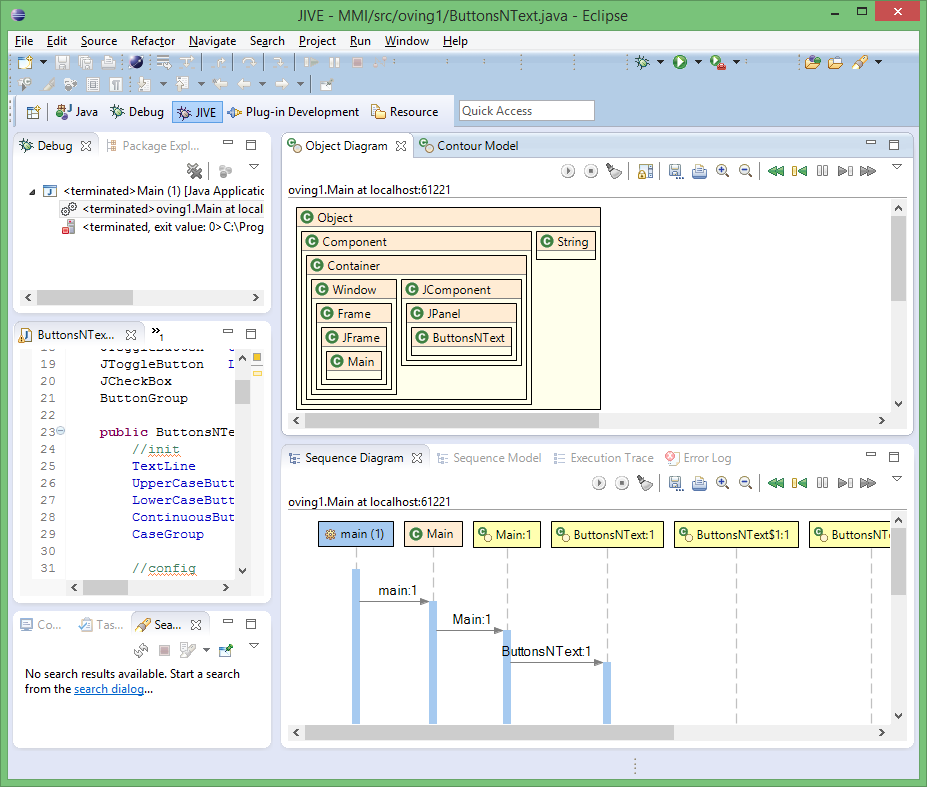
\includegraphics[width=\textwidth]{jivePerspective3}
	\caption{The JIVE perspective in Eclipse}
	\label{fig:jivePerspective}
\end{figure}
As mentioned in the prestudy, JIVE installs as a plugin in the eclipse IDE, adding another perspective in the environment shown in \autoref{fig:jivePerspective}.
The default views shown in this perspective are the "object diagram" and "sequence diagram" views, making the diagrams generated during debugging JIVEs two most apparent features.
The diagrams are updated according to the current state of the debugged program, so that the backtracking functionality allows you to see the entire execution graphically step-by-step.
The other views provided by JIVE are as follows: "contour model", "sequence model", "execution trace" and "search".
~\\

\begin{figure}[H]
	\centering
	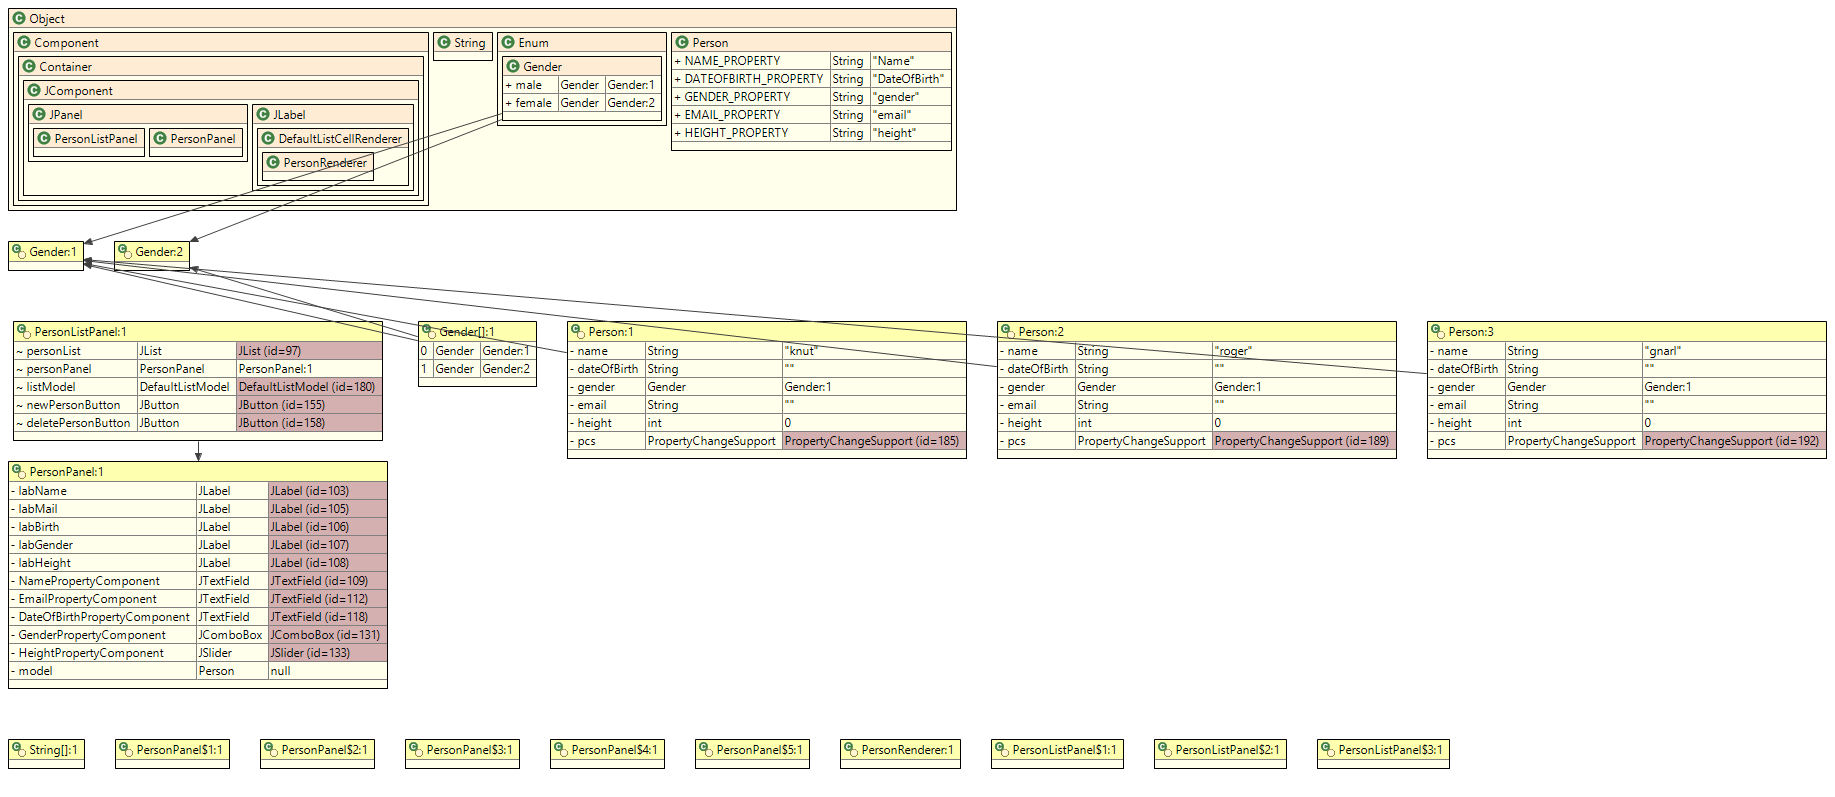
\includegraphics[width=\textwidth]{MMI-Oving4-ObjectDiagInit}
	\caption{A contour diagram generated by JIVE}
	\label{fig:oving4ContDiagInit}
\end{figure}
The object diagram-view shows the current state of the program by using a contour-diagram.
Contour-diagrams, as shown in \autoref{fig:oving4ContDiagInit}, are based on an old technique to give semantics to Algol-like languages.
The basis has been extended to support modern concepts, such as object-oriented programming.
Objects are represented by a box, or contour.
Within the contour, the objects variables are shown, with name, type and value.
The contour also uses arrows to point at other contours that are related, e.g. an other object representing the value of a variable, or an enumerator.
Inheritance is shown by putting the contour of an object within the contour of the extended object. 
Object instances are kept separate from the contours representing inheritance, but will have relational links when necessary.
Method calls are also represented in the diagram, in their own contours, linked to the calling object.
JIVE offers to hide some of the information, such as inheritance or the composition of objects, in order to make the diagram smaller, and easier to read.
Something that can be especially useful when working with larger programs, with many objects and relations.
Visibility is aided by the use of colors to highlight specific elements of the diagram, such as variables bound to objects, and method-calls.
~\\

\begin{figure}[H]
	\centering
	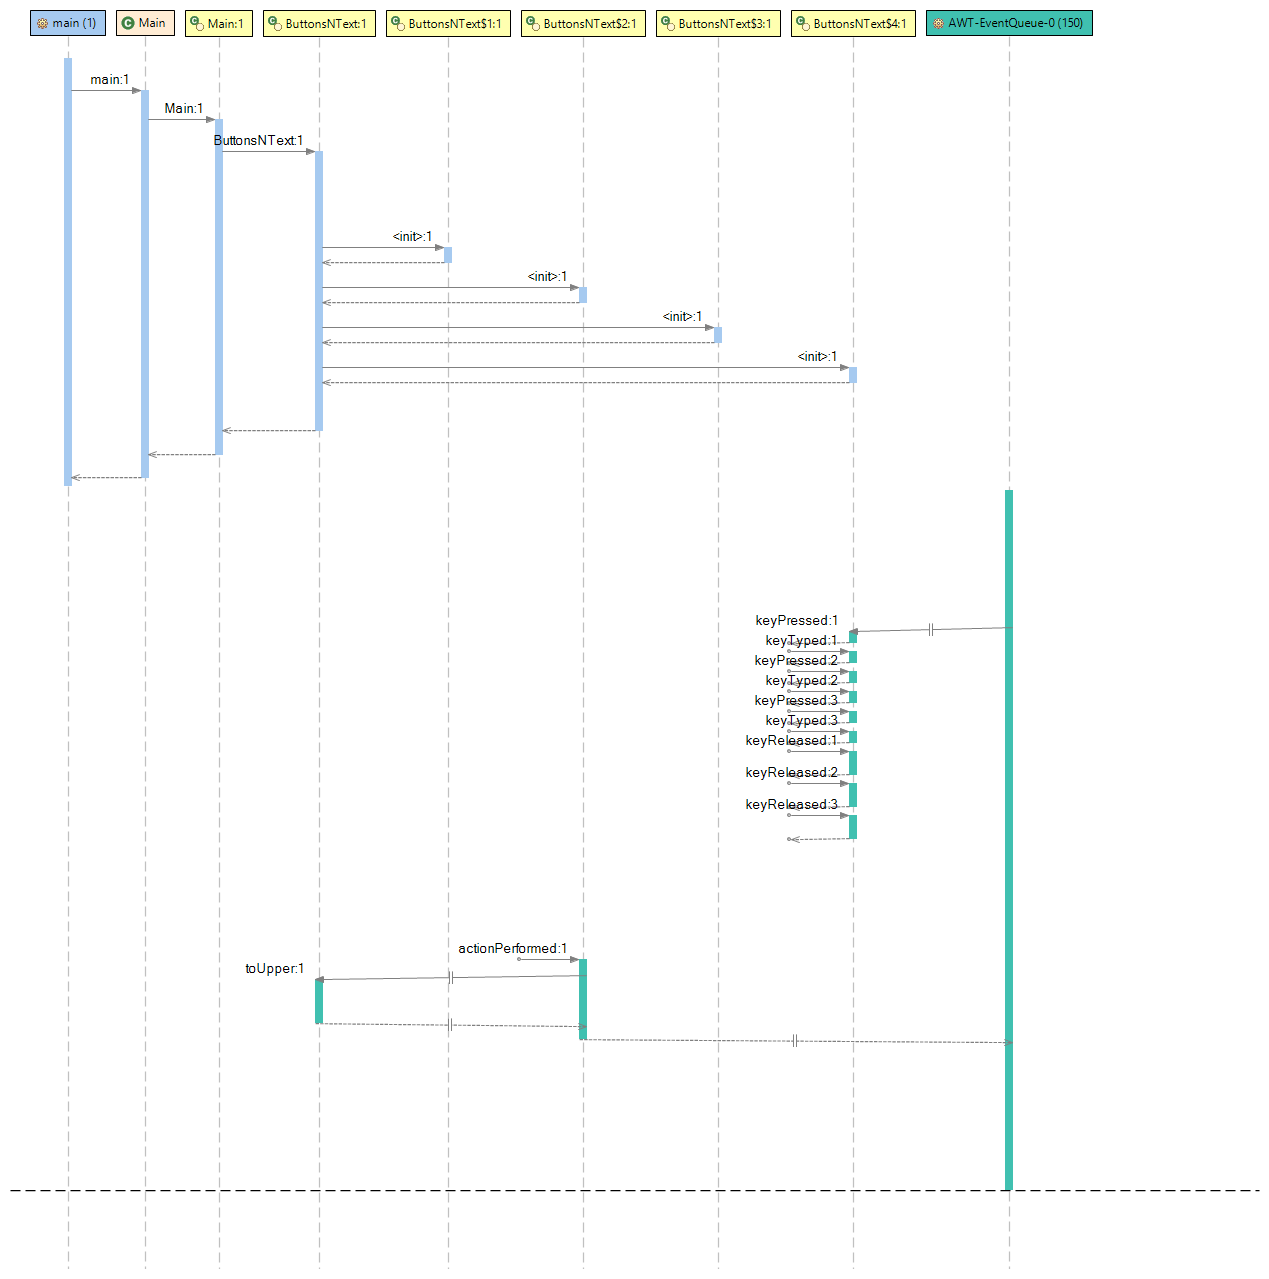
\includegraphics[width=\textwidth, trim=0 0cm 0 0, clip]{MMI-Oving1-SequenceDiag}
	\caption{A sequence diagram generated by JIVE, while running an instance of MMI-Exercise 1}
	\label{fig:oving1SeqDiag}
\end{figure}
The sequence diagrams, shown in \autoref{fig:oving1SeqDiag}, are fairly standard, with threads and objects represented by boxes on a row at the top, each with a vertical life-line.
The actual sequence is shown with a thicker lifeline, with arrows representing method-calls.
In order to differentiate the threads where the execution is happening, the sequences are colored with the same color as the thread- box the sequence originates from, regardless of witch objects and methods are involved.
In \autoref{fig:oving1SeqDiag}, one can clearly see the two colors representing the main- and the AWT-event-thread, and how elements in the diagram are colored by their parent thread.
\begin{figure}[H]
	\centering
	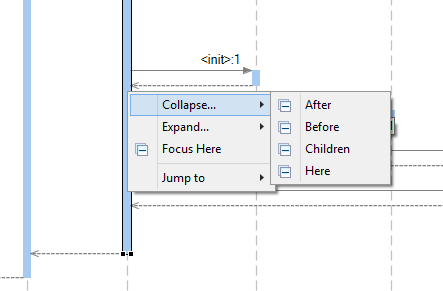
\includegraphics[scale=0.9]{seqRightClick}
	\caption{The sequence diagram right click menu}
	\label{fig:seqRightClick}
\end{figure}
Right-clicking on a lifeline offers the ability to collapse method-calls originating from that lifeline in order to hide unnecessary information, shown in \autoref{fig:seqRightClick}.
The collapse-menu offers four options when used on the lifeline of an object: after, before, children and here.
Before and after collapses lifelines that occurred before or after the selected event, at the same depth in the sequence-tree.
Children collapses all events that are children of the selected event, while here collapses the selected event.%figurer!
Right clicking on an object instance at the top of the diagram also offers to collapse that objects entire lifeline, the result of which can be seen in \autoref{fig:seqOving4Collapse}.
The same options are of course available for expanding collapsed elements.
Right-clicking also offers to set the execution-state via the jump-option, updating the contour-diagram and -model to show that state.
~\\

\begin{figure}[h]
	\centering
	\begin{subfigure}{\textwidth}
		\centering
		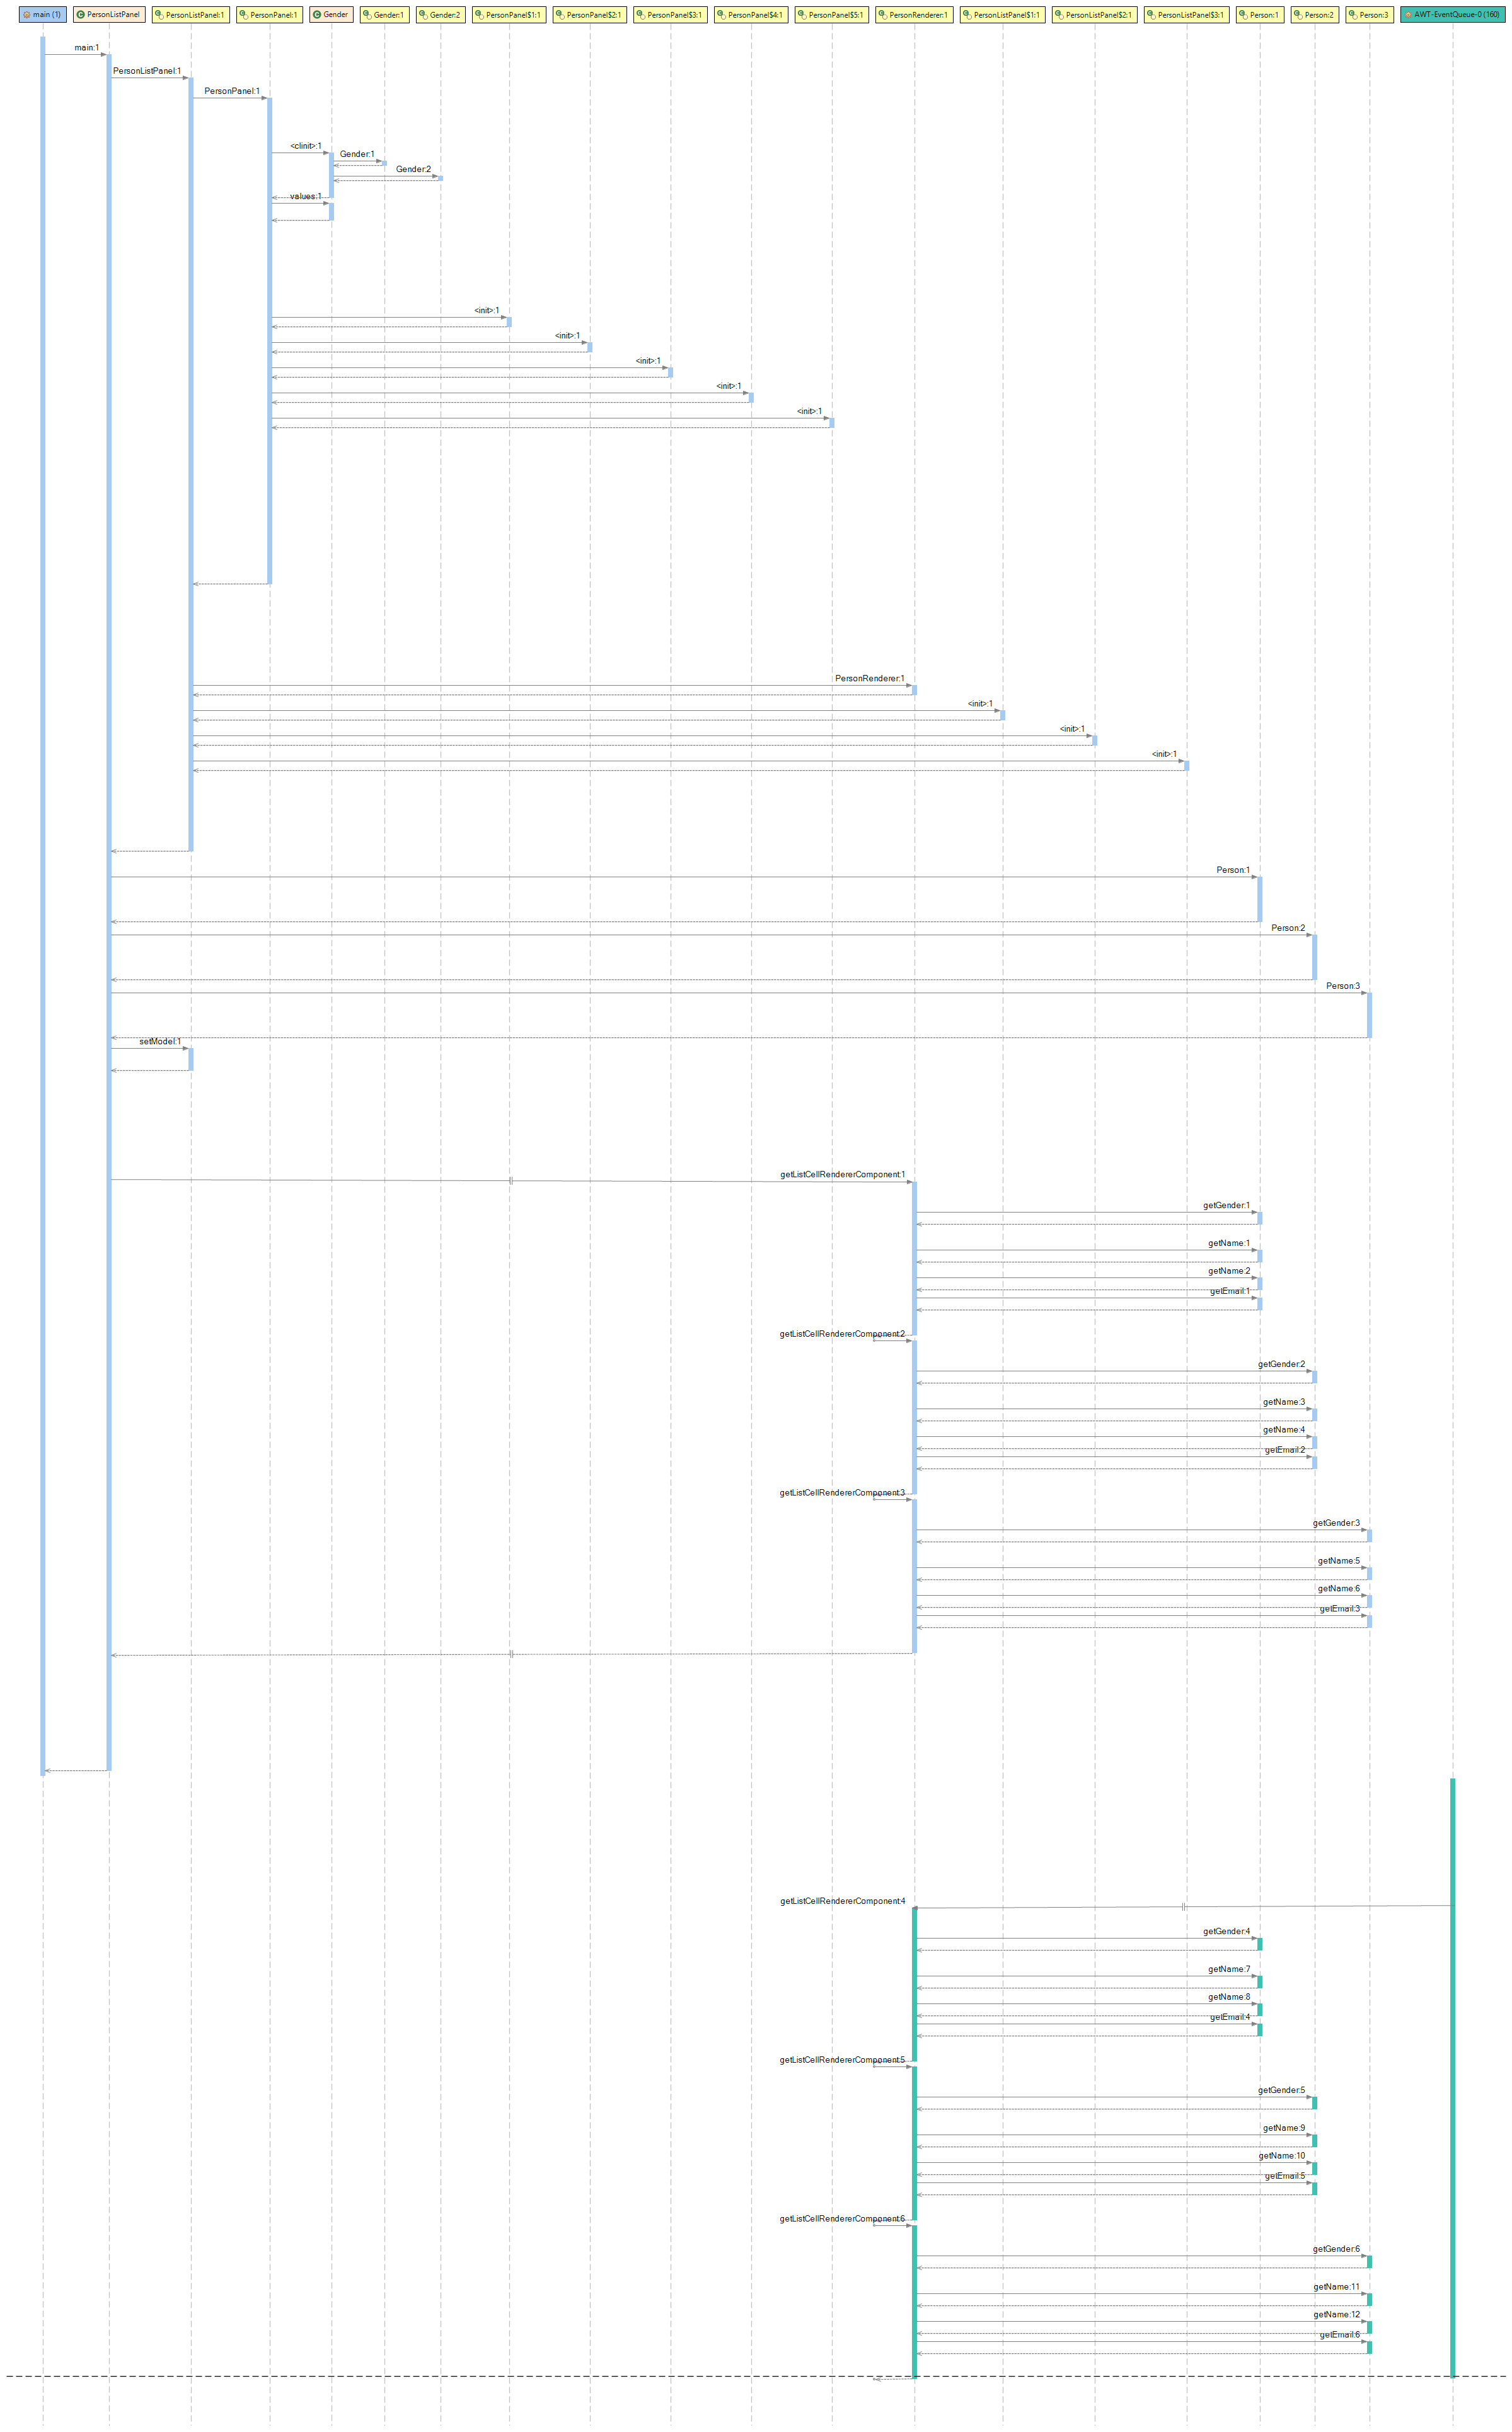
\includegraphics[width=\textwidth, trim= 0 40cm 0 50cm, clip]{MMI-Oving4-SequenceDiagInit}
		\caption{Normal}
		\label{fig:seqOving4CollapseA}
	\end{subfigure}
	\begin{subfigure}{\textwidth}
		\centering
		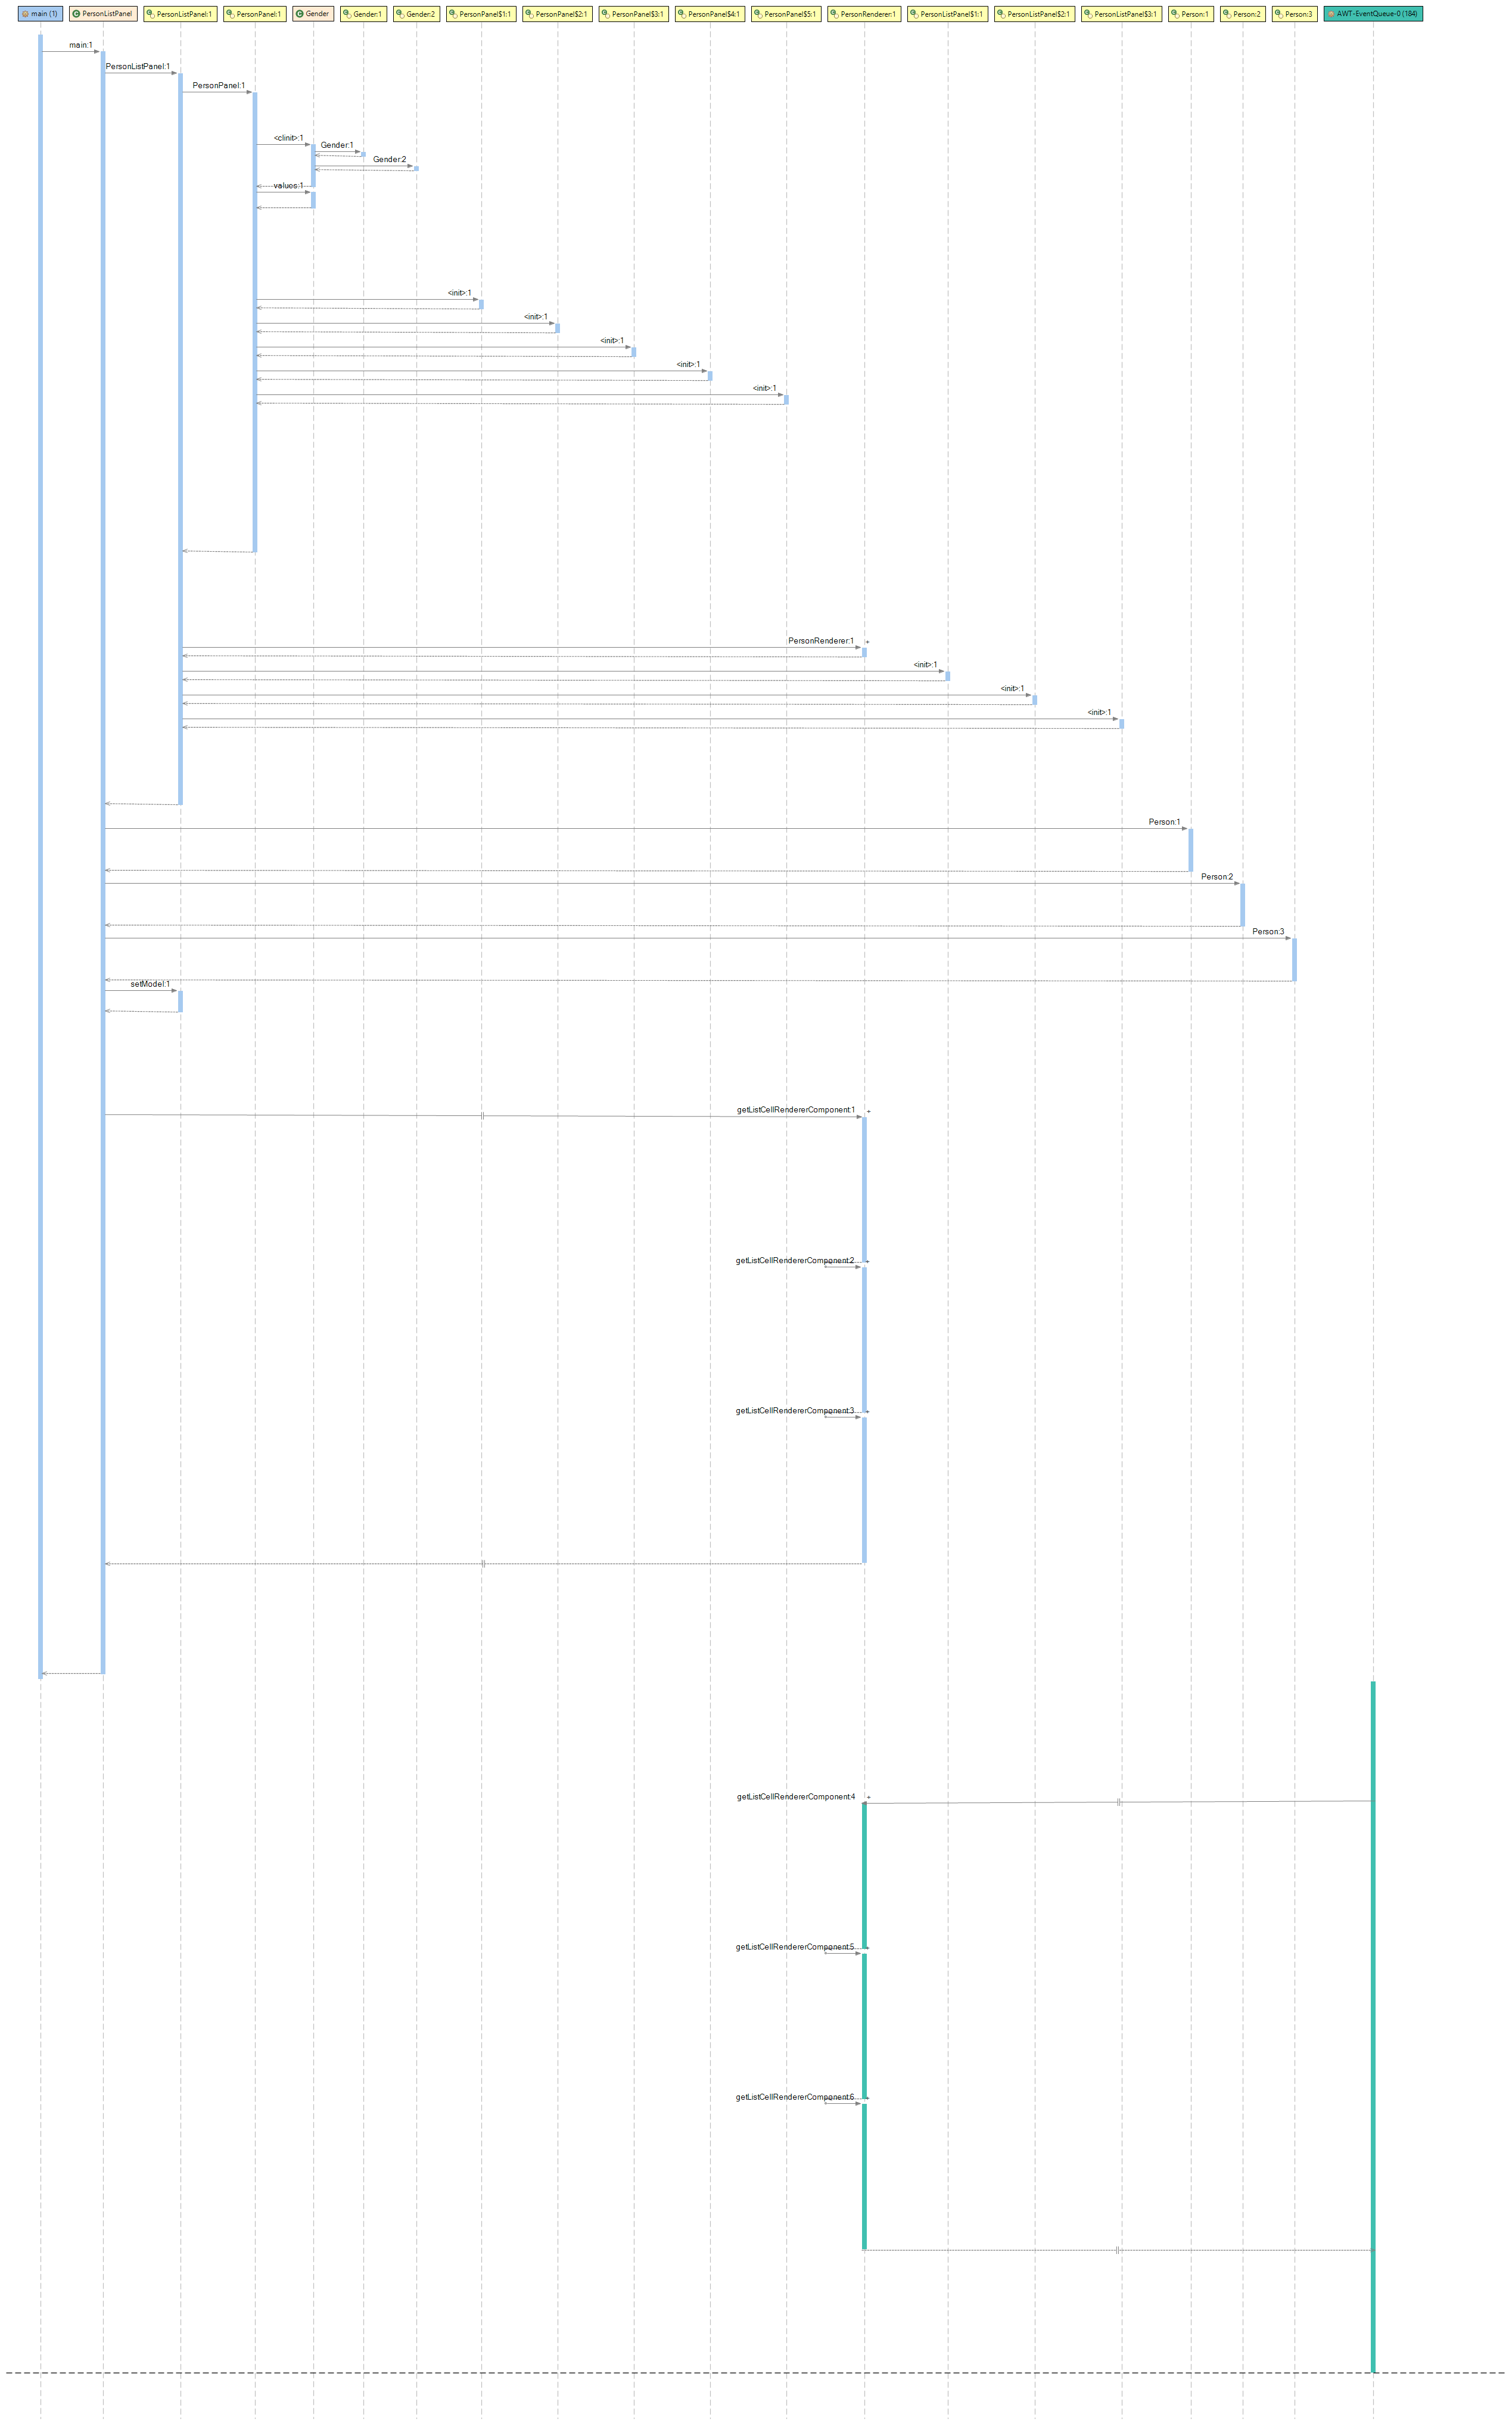
\includegraphics[width=\textwidth, trim= 0 48cm 0 50cm, clip]{MMI-Oving4-SequenceDiagInitCollapsed}
		\caption{Collapsed}
		\label{fig:seqOving4CollapseB}
	\end{subfigure}
	\caption{Normal and collapsed section of a sequence diagram}
	\label{fig:seqOving4Collapse} 
\end{figure}

Both of the diagrams can be saved as a high-resolution image at any time, so that one can look at diagrams from earlier runs, instead of being forced to view them through JIVE.
This also helps to visualize any changes made to a program, and to see what the effects are on the program flow.
They also share the ability to zoom in and out, further helping with the handling of larger diagrams.
~\\

Closely related to the diagrams, is the ability to quickly jump backwards and forwards between execution states.
This is enabled by the trace-log, containing an entry for every single event that occurs during execution of a program.
Each event is assigned an identifying number, in ascending order, and information about thread, type, caller, target, and the location of the source-code is stored.
The log is used as the basis for the models that make up the diagrams, and can be saved as both XML- and CSV-files for later use.
As mentioned in the Prestudy, logging every event has a significant impact on run-time performance, limiting the size of the programs that can be used in a meaningful way.
On the other hand, it allows the almost instant jumping between recorded states, as opposed to techniques that save a snapshot at predefined intervals, requiring the program to be run from the snapshot-state to the desired one, even if it is just a single step backwards.
~\\

The model-views each display an alternate view of their respective diagrams.%figur
They show the data-model representing the diagrams in a hierarchical structure, much like the organization of files and folders.
Right-clicking on an event in the sequence model allows you to set the execution state to that event, and have the diagrams updated accordingly.
Clicking on elements in the contour-model allows you to inspect the values of objects and their variables.
~\\

Finally, the trace-log enables the use of queries to search for specific events in the execution.
The queries are presented through a new tab in the eclipse search-window as seen in \autoref{fig:jiveSearchPanel}, easily accessible through the search-view, and comes with several pre-defined templates to simplify searching.
For example, searching for when a certain variable gets a certain value, only requires the user to specify the variable-name, its parent, and the value.
\begin{figure}[H]
	\centering
	\includegraphics[width=\textwidth]{jiveSearch}
	\caption{The JIVE search panel}
	\label{fig:jiveSearchPanel}
\end{figure}
~\\

\subsection{Shortcomings of JIVE}\label{jiveShortcomings}

Even though JIVE offers several useful features, there is still room for improvements, both for general use, and more tailored towards development of graphical interfaces, as is the focus of the MMI-course.
~\\

The diagrams are possibly the most useful feature of JIVE, showing a lot of information in an understandable way, and offering some useful interaction.
But there is still room for improvement:
Inner types are displayed with their automatically generated, and fairly anonymous, name unless given a proper name in code.
By default, most of the classes defined by the JRE itself are ignored, omitting potentially important information in GUI-applications.
For the sequence-diagrams, it is naturally not important no show the internal behavior of every object, but they are also hidden in the contour-diagram.
Related to this, is the lack of visual connections between standard-objects, and for example instances of listeners added to them.
More related to the target group for this project, is a lack of differentiation between the different object-types in typical graphical architectures.
Especially MVC, whitch is a major focus of the MMI-course, has certain distinct types that are more important than others.
~\\

The sequence-diagrams can quickly become huge and hard to navigate, and the zooming function has very few levels outward, as well as leaving all text to small to read when zooming out.
Additionally there does not seem to be any way to vertically compact the sequence-diagrams, making them unnecessarily long in cases where calls to ignored or hidden methods are being made.
For instance when horizontally collapsing large parts of the diagram, leaving the parent lifeline at the same length as before, as can be seen in \autoref{fig:seqOving4CollapseB}.
Some of the papers on JIVE mention regex-folding,that could be used to substitute a series of events with a single new event, but it is nowhere to be found in the latest version of the plugin.
~\\

Another potential for improvement is the process of stepping through recorded states, which currently requires manual interaction for each step, making complete replays of an execution infeasible due to the massive number of events recorded even for simple programs.
~\\

The search-view, while useful, is very strict in terms of what it looks for.
For example, searching for the creation of an object requires its full name, including packages, so searching for creations of JButton-instances would require a search for javax.swing.JButton.
~\\

\subsection{Suggestions for improvement}\label{jiveSuggestions}

Based on the mentioned shortcomings, the following improvements are suggested.
~\\

The ability to detect an inner type with a generic name, and display its parent type in the diagrams instead of its own.
This will make, among others, listener-heavy programs much more understandable as one can see what kind of listener each object is, instead of guessing, based on when it is invoked in the sequence-diagram.
Further helping the same situation, is to visually link listeners to the objects they are added to, in the contour-diagram, making it clearly visible which object is being listened to by the different listeners.
A crude visualization of these two changes, compared to the original, can be seen in \autoref{fig:contOving4Changes}.
~\\

Finding ways to highlight the different parts of e.g. an MVC-architecture, making it clearly visible which objects make out the models, views and controllers, may further help the understanding of a program.
But such highlighting must be balanced in order to not create a visual chaos of different colors.
Adding symbols instead of colors might be a better solution, both maintaining the current color-scheme, and adding new information.
The coloring, and naming of inner types should apply to both of the diagrams.
~\\

\begin{figure}[h]
	\centering
	\begin{subfigure}{\textwidth}
		\centering
		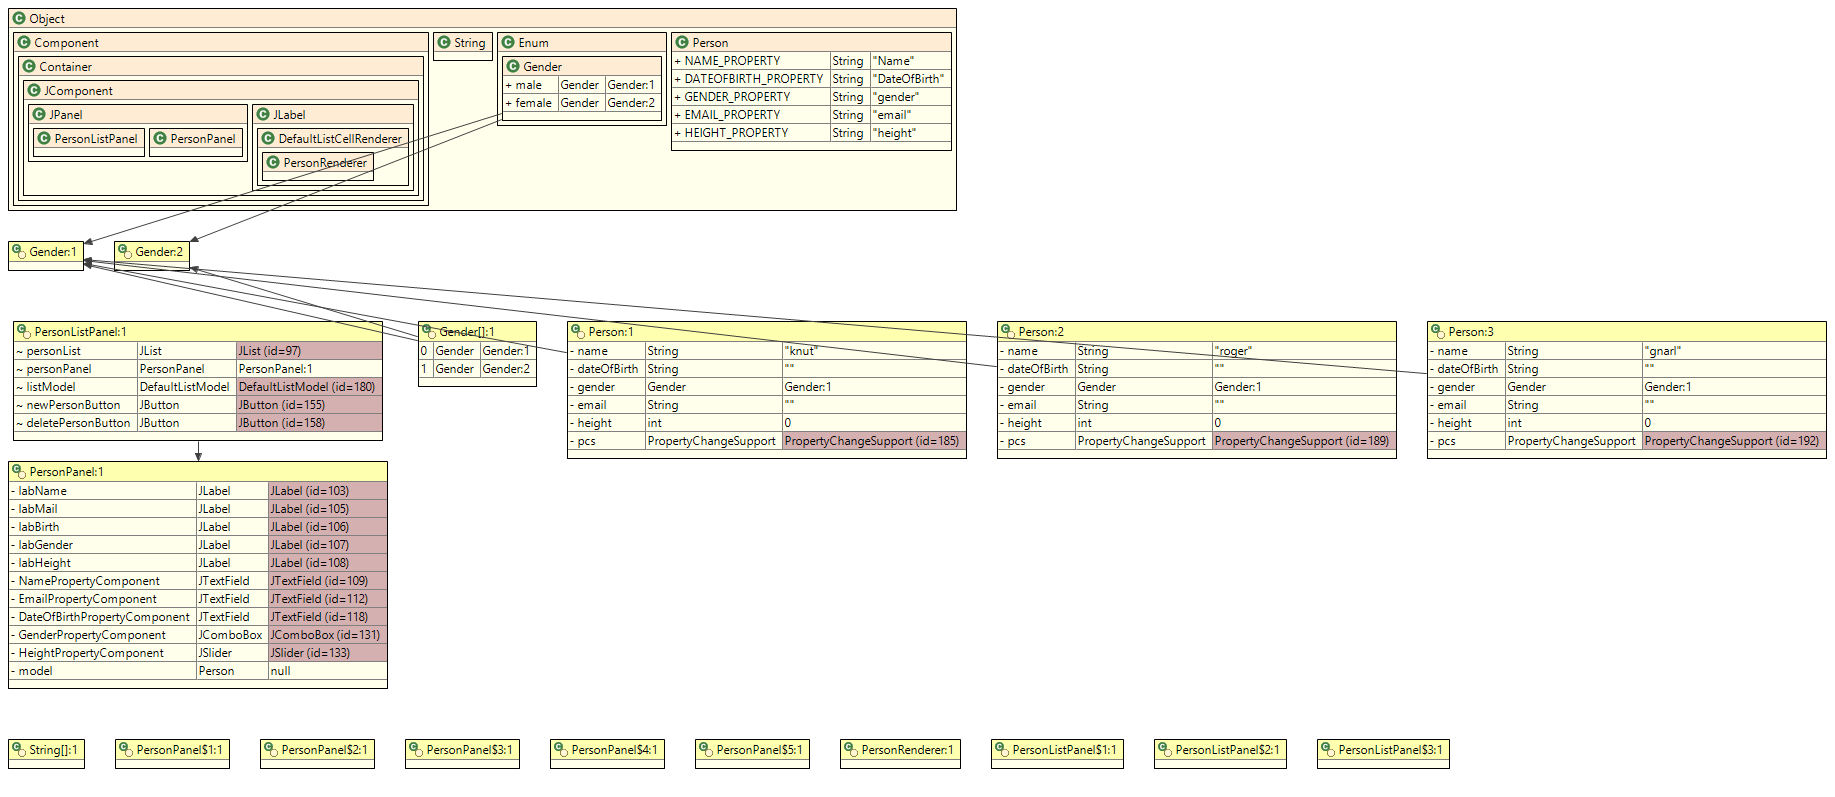
\includegraphics[width=\textwidth, trim= 0 0 0 0, clip]{MMI-Oving4-ObjectDiagInit}
		\caption{Original}
		\label{fig:contOving4ChangesA}
	\end{subfigure}
	\begin{subfigure}{\textwidth}
		\centering
		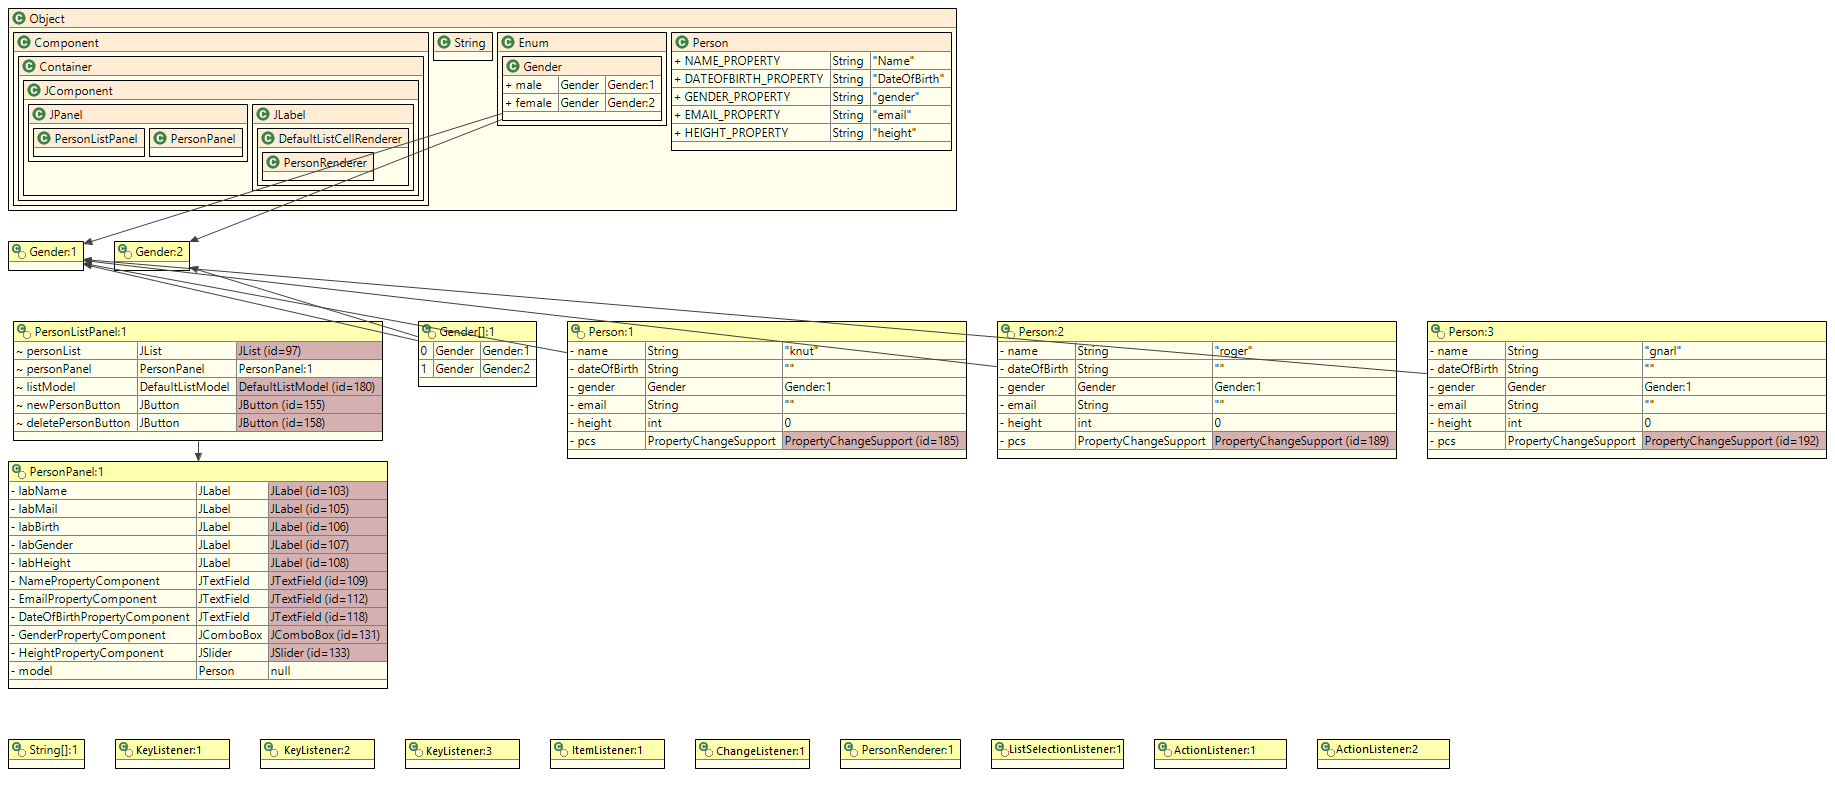
\includegraphics[width=\textwidth, trim= 0 0 0 0, clip]{MMI-Oving4-ObjectDiagInit-edit}
		\caption{Changed naming of inner types}
		\label{fig:contOving4ChangesB}
	\end{subfigure}
	\begin{subfigure}{\textwidth}
		\centering
		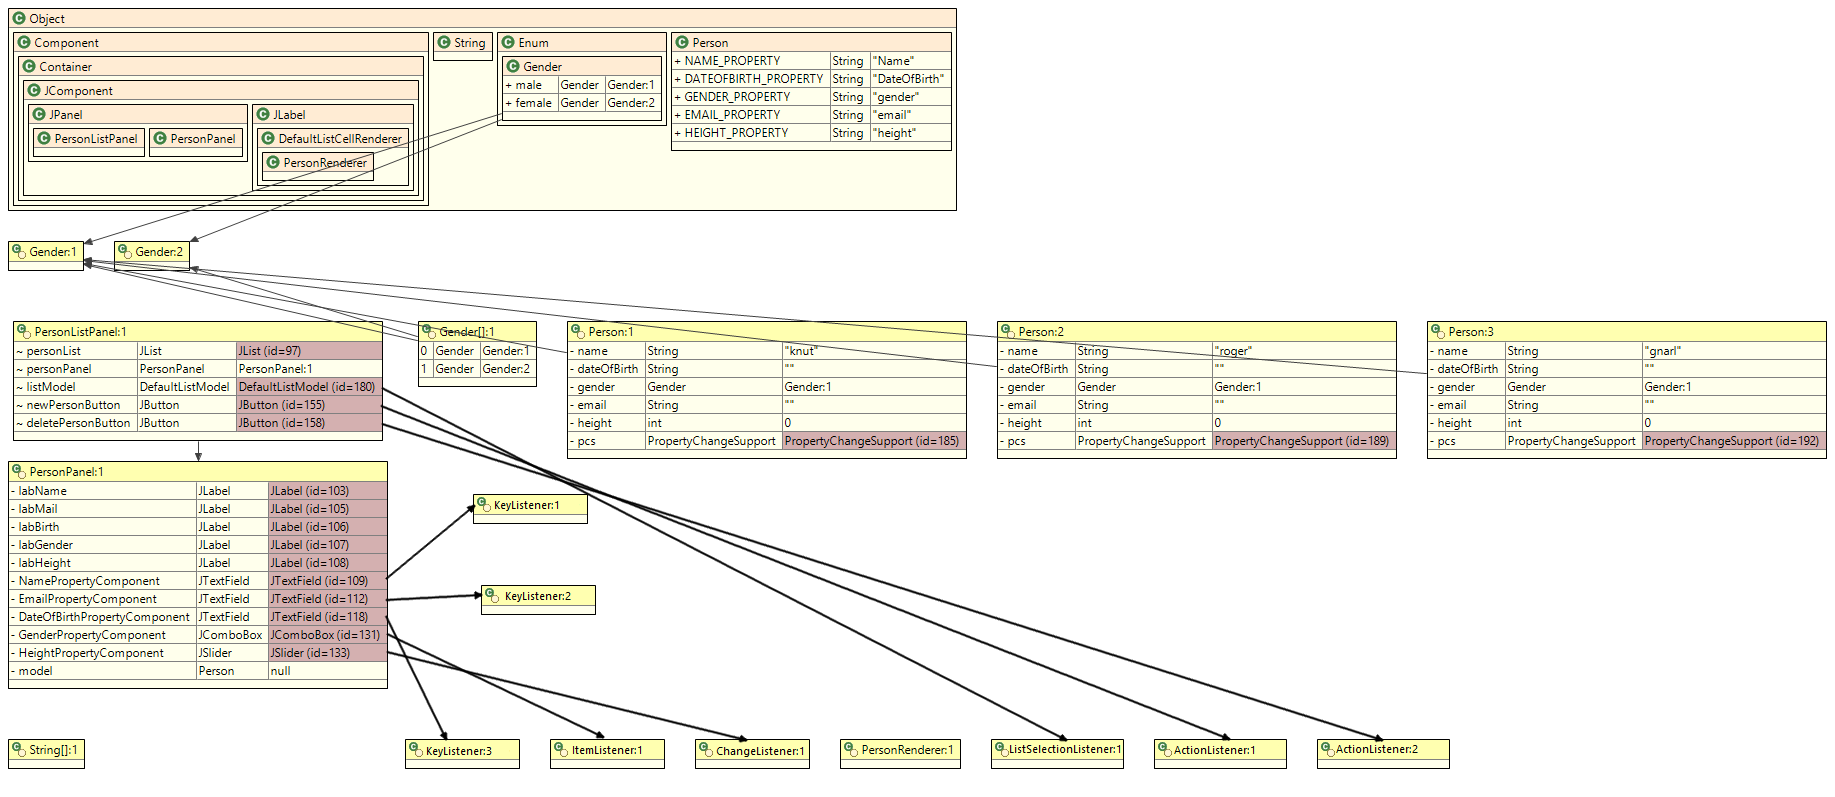
\includegraphics[width=\textwidth, trim= 0 0 0 0, clip]{MMI-Oving4-ObjectDiagInit-edit3}
		\caption{Listeners connected to the object listened to}
		\label{fig:contOving4ChangesC}
	\end{subfigure}
	\caption{Crude comparison of suggested changes to the contour diagram}
	\label{fig:contOving4Changes} 
\end{figure}

Exploring changes to the default exclusion-filter, in order to provide more useful information out of the box, is also an option.
This will provide a better experience for certain scenarios, but may be useless in other cases by providing too much unnecessary information.
A way to easily switch filters by defining presets might be preferable.
The filter might also be extended to support both exclusion and inclusion, allowing a more fine-grained selection of interesting classes.
For example ignoring the entire javax.swing-package, apart from a few selected classes that are relevant.%eksempel?
~\\

Allowing more ways to interact with the diagrams, e.g. hiding elements or compressing sequences, should improve usability for larger programs and longer runs.
In the case of exploring events triggered by a listener, the ability to isolate the involved objects, and reorder the diagram could be very useful, providing a clean view of a smaller series of events.%figur
This function should be accessed by right clicking on the topmost event that is desired, and selecting a "view isolated" option.
Whether the isolated view should appear in a new eclipse view, or simply modify the existing view of the sequence diagram,  is something that should be determined by user-testing.
~\\

Stepping through the recorded states is, as mentioned above, cumbersome.
While there are quick and easy ways to jump straight to any interesting state, it may also be interesting to view a playback of a part of, or the entire execution.
This would allow an easier way of observing changes happening in a program.
~\\

Searching can be improved by relaxing the requirements for for search-terms.
For instance by allowing partial class names, or substrings in general.

\section{Implemented changes}\label{jiveImpl}%hva ble gjort, hvordan bruke funksjonene. Ikke så mye om hvordan. begrunne prioriteter?
~\\

%identifisering av instansierte grensesnitt, lambdaer og abstrakte klaser
The first change to be implemented was the identification and presentation of instantiated interfaces, which are now displayed in the diagrams with an appropriate icon, as well as being labeled with the interface it implements, instead of the generic class name that it is assigned by default.
An example of this is shown in \autoref{fig:JiveNewIcon}
This function was also expanded to identify and label instances of abstract classes, and the lambda-expressions that were introduced with Java 8.
In order to still allow the actual class name to be visible, the tool-tip shown when hovering the mouse pointer over an object remains unmodified, showing the actual class name and icon.
\begin{figure}[H]
	\centering
	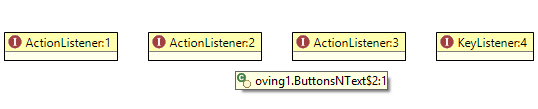
\includegraphics[width=\textwidth]{UIJiveInterfaceIcon}
	\caption[A view of how instantiated interfaces are shown after the modification.]{A view of how instantiated interfaces are shown after the modification. Also shown, is the tool-tip text for the second instance from the left. Originally, they would be labeled as 'ButtonsNText\$1:1', 'ButtonsNText\$2:1' and so on, with the green class-icon.}
	\label{fig:JiveNewIcon}
\end{figure}
~\\

%utvidelse av filteret
The filtering function was expanded with the ability to specify packages that are not to be excluded from the execution model, as suggested in \autoref{jiveSuggestions}.
Adding a package to be included is as simple as adding a `+' in front of the package-name when adding it to the filter.
As an example, the default filter excludes the javax package, and any subpackages that are not specifically listed with a `+' in front.
When adding the line `+javax.swing.*' in order to let swing components through the filter, one will let every subpackage of 'javax.swing' though the filter as well, which is the intended design.
Unfortunately, there are a lot of classes in both swing, and its subpackages that are not used directly when writing swing-programs, and a user will have no interest in seeing these in the diagrams.
This can result in very poor performance, as unnecessary events are logged, and cluttered diagrams, but can be handled by adding the unwanted classes to the filter for exclusion.
Depending on the package in question, the amount of extra items added to the filter can become quite large, and identifying all unwanted classes and subpackages may take hours at worst.
One weakness in the filter, related to the problem of unwanted packages, is that due to its design, allowing the contents of a package, will also allow any classes that are contained directly within the parent package, as this also has to be removed from the internal list of exclusions that make up the filter.
This is not a big problem in the case of `javax.swing', as the `javax' package does not contain any classes, but there are definitely other packages that will show this behavior.
~\\

With an appropriate filter, the connection between listeners and the objects they listen to should become visible, via the existing object-containment-links, given that the listener-field is actually visible.
An unfortunate behavior of JIVE is that only the fields defined within a class are visible in the figures representing instances of that class.
%TODO test for å være helt sikker
Any inherited fields are not shown, and this is unfortunately the case for many UI-components in the swing-framework.
The quick solution to this problem, simply showing all inherited fields, would result in a large amount of useless information, cluttering the diagram, and hiding the useful information.
In lack of a good solution, and with a desire to not make large fundamental changes, preferring minor adjustments that use the existing framework in better ways.
Assuming that the listener-field is visible, this would in most cases be a list of listeners, and so the filter would also need to allow that type of list through.
As there are a large amount of lists in use behind the scenes in a graphical program, this would be another source of unnecessary clutter.
The filter itself is likely to become very large due to the extra exclusions needed to hide unwanted classes, as a consequence of letting something through.
~\\

There is currently no easy way to quickly swap the entire filter for another one, but the filters are stored in eclipses launch configuration files.
These configurations are stored as XML-files, and can be easily modified in any text editor.
By managing these files directly, a user can quickly swap the entire filter, copy it to another launch-configuration file, or share it with others.
After modifying these files, Eclipse requires a restart to detect the changes, adding to the time and effort required to make any changes this way.
This is of course not a good way of handling the issue, and ways of improving this should be explored in the future.
~\\

%isolert visning av sekvens
The isolated view was implemented as a separate view-tab, and does what was proposed in \autoref{fig:seqOving4IsolatedMock}: it displays the events caused by the selected event, and hides everything else.
\autoref{fig:MMI-oving4-SeqIsoDiag-AWT-Event-Thread} shows what \autoref{fig:seqOving4IsolatedMock} looked like after the modification.
\autoref{fig:MMI-oving4-SeqIsoDiag-valueChanged} shows a similar, but slightly more complex situation in the isolated view.
By right clicking on an event in the regular sequence diagram, and selecting the `Isolated view' option, shown in \autoref{fig:UISeqRightClickNew},  the isolated view is triggered.
It is also possible to further focus on a part of the diagram from within the isolated view, by right clicking on the desired event, and selecting the `Isolated view' option again.
All of the functionality from the regular sequence diagram has been retained in the isolated view, so that the only difference is what parts of the execution are visible.
\begin{figure}[H]
	\centering
	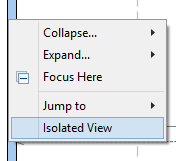
\includegraphics{UIseqRightClickNew}
	\caption{The new 'Isolated view' option.}
	\label{fig:UISeqRightClickNew}
\end{figure}
~\\
\begin{figure}[H]
	\centering
	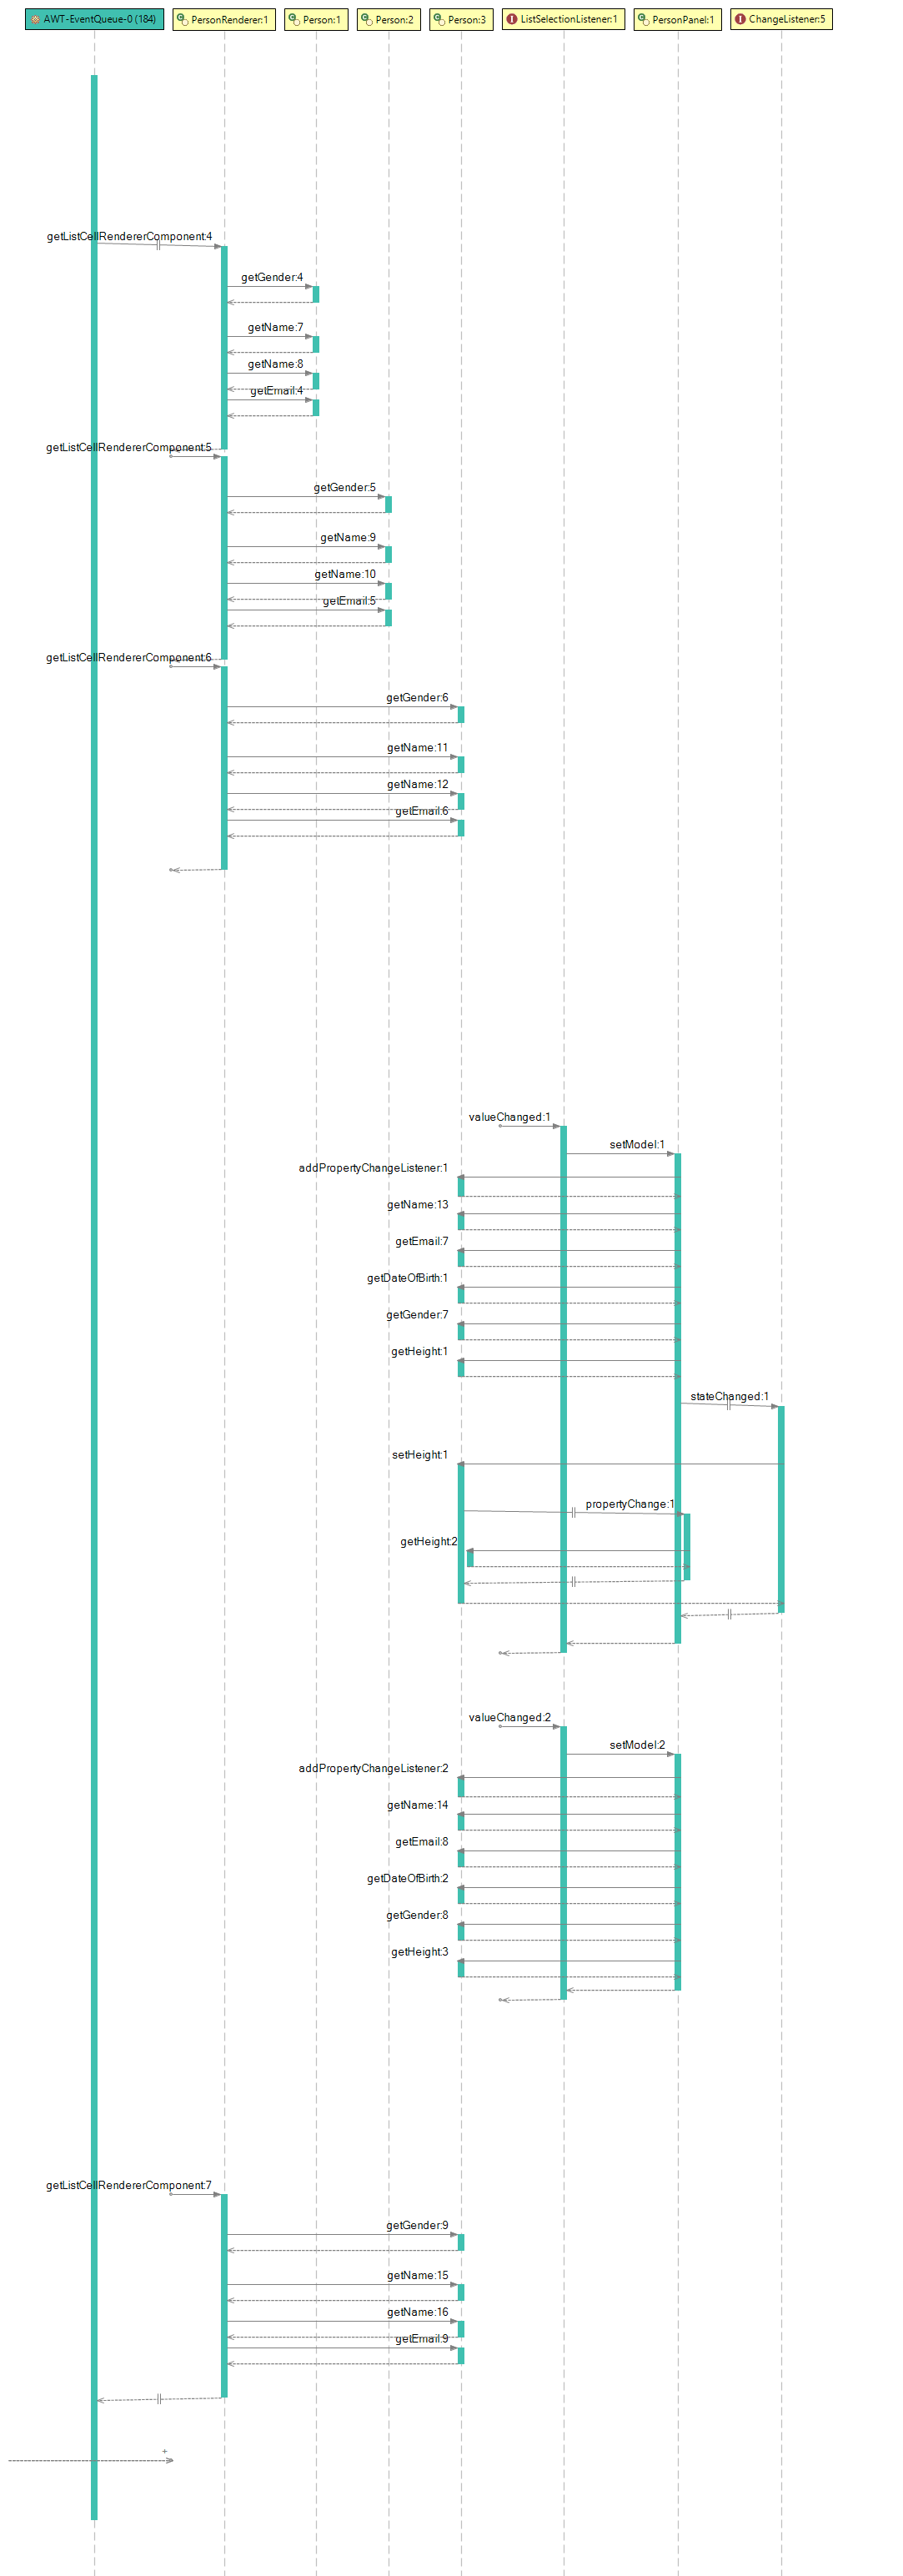
\includegraphics[width=\textwidth, trim= 0cm 50cm 0cm 0cm, clip]{MMI-oving4-SeqIsoDiag-AWT-Event-Thread}
	\caption[How \autoref{fig:seqOving4CrossLines} looks in the isolated view.]{How \autoref{fig:seqOving4CrossLines} looks in the isolated view. The three last elements shown on the top are referred to in parts of the diagram not shown. This view was achieved by selecting the 'AWT-EventQueue' lifeline for the isolated view.}
	\label{fig:MMI-oving4-SeqIsoDiag-AWT-Event-Thread}
\end{figure}
~\\
\begin{figure}[H]
	\centering
	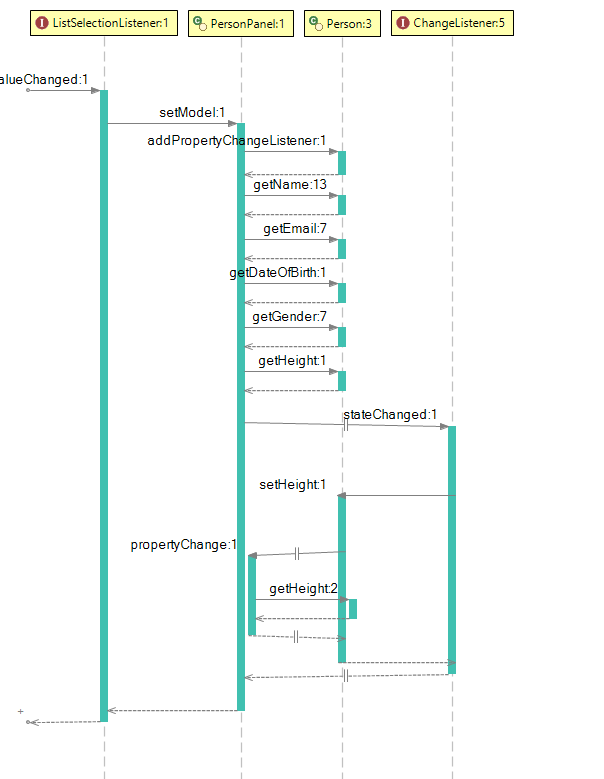
\includegraphics[width=\textwidth, trim= 0cm 0cm 0cm 0cm, clip]{MMI-oving4-SeqIsoDiag-valueChanged}
	\caption{Another example  of the isolated view, showing a significantly reorganized diagram.}
	\label{fig:MMI-oving4-SeqIsoDiag-valueChanged}
\end{figure}
 ~\\

%mer avslappede søkekrav - er ikke utført for alle typer søk, er det verd å nevne i det hele tatt?
The searching functionality was relaxed by allowing partial matches, and disabling case sensitivity.
While relaxing the search may cause false positives, a user should be able to identify such cases quickly, or at least identify the results they were looking for.
The fact that partial matches and case insensitivity is the standard behavior in most search-engines, sets an expectation for the behavior of the search within JIVE.
Unfortunately, due to the existing implementation consisting of separate searching- and matching-methods for each search type, not all searches were updated to this relaxed state.

%hvorfor ble ikke alle forslag impementert? - tid for å bli kjent med jive, eclipse-plugins

\chapter{Evaluating usefulness}\label{jiveEval}

This chapter will look at the external evaluation of \gls{jive} and the implemented changes, providing details on both the execution of the evaluation, and the results that were acquired.

\section{The test}\label{jiveEvalTest}
%mer konkret om hva som ble spurt om, spesifikke spørsmål
In order to evaluate both the usefulness of \gls{jive}, and the changes that were implemented, the evaluation was performed individually with a small group of six students.
The participants were initially recruited through a request sent to everyone that were taking a second-year course that is mandatory for those who follow the informatics program.
This group was selected as they were matching the target group outlined in \cref{introduction}.

After only getting a single response, another request was sent to the students' association of the computer science program, bringing in the five remaining participants.
The latter group were all in their third year, and had already finished the \gls{hci}-course the previous semester.
This meant that they were familiar with the example programs, and had some knowledge of the MVC-pattern and how it behaves in Java-swing.
While this excluded the experiences of someone completely unfamiliar to these concepts, it did give the insight of relatively fresh experiences, as the participants remembered what they were finding hard to understand during the course.

During the test, the students were given a demonstration of the main features of \gls{jive}, using implementations of the first and the last exercise of the \gls{hci}-course as examples.
After getting familiar with \gls{jive}, they were shown the modified version, focusing on the new and modified features that were implemented.
They were then asked questions about how easily they understood the diagrams, and how useful they found the changes to be.
As well as whether the performance trade-off was acceptable for occasional use, if they could see themselves using \gls{jive}, and if so, in what situations.

The example programs both consisted of a simple user interface in Swing, implementing the \gls{mvc} pattern.
Exercise 1 consists of a text field and two buttons to transform the text entered in that field to either uppercase or lowercase, and with an option to continually transform as new text is written.
Exercise 4 is an application that manages a simple list of people.
The interface it presents is split between a list of people, and a set of text fields to enter information about the selected person, as well as buttons to create new, and delete existing people.
Both of these programs, shown in \cref{fig:MMI-Oving-UI}, were relatively simple, with few events following directly from user interaction, and as such, should have a limited performance reduction when used with \gls{jive}.
More complex programs are likely to suffer a greater performance impact from \gls{jive}, but are also out of the scope for the \gls{hci}-course.


\begin{figure}[H]
	\centering
	\begin{subfigure}{\textwidth}
		\centering
		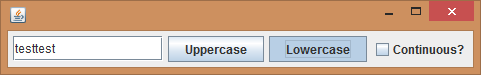
\includegraphics[width=\textwidth]{MMI-Oving1-UI}
		\caption{\gls{hci}-exercise 1.}
		\label{fig:MMI-Oving1-UI}
	\end{subfigure}
	~\\
	~\\
	\begin{subfigure}{\textwidth}
		\centering
		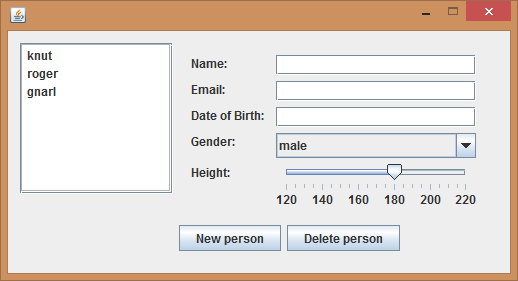
\includegraphics[width=\textwidth]{MMI-Oving4-UI}
		\caption{\gls{hci}-exercise 4.}
		\label{fig:MMI-Oving4-UI}
	\end{subfigure}
	\caption{The two example programs used in the evaluation.}
	\label{fig:MMI-Oving-UI}
\end{figure}

\section{Results}\label{jiveEvalResults}

%nytte av diag
The evaluation resulted in mostly positive feedback, with every participant seeing some kind of use for a tool like \gls{jive}.
Of those in their third year, only one participant did not consider the use of diagrams to understand code to be useful.
In his experience, he learned just as well from reading the code directly, and building his own mental model of the program structure, but as he preferred simple text editors to \gls{ide}s, he could be considered to be outside of the target demographic.
On the other hand, he did recognize the usefulness of \gls{jive} as a tool to create documentation, and for presenting his own work to other participants in a project.
The rest of the participants shared the view that \gls{jive}, or a similar tool, could have been very useful when trying to understand the connection between \gls{gui} elements, listeners, and the actions that are triggered by them.
A few specifically mentioned that they found that connection to be difficult to understand.
One of them also had experiences as a student assistant, and recognized \gls{jive} as a tool that could give students a needed insight into what is going on in their programs.

The diagrams themselves were found to be both sufficiently detailed, and easy to understand, showing the available information in a simple and structured manner.
The tendency for the diagrams to grow large and unwieldy did become a problem, especially when running with the less restrictive filter that was showing more of the Swing-internals.
When hiding everything but user-created classes, the diagrams remained at an acceptable size, although the sequence diagram got quite long after a while.

%nytte av endringer
The implemented changes were generally well-received, with the ability to view a subsection of the sequence diagram in the isolated view being the most preferred change.
The changes to the filtering mechanism, while useful, were found to still be somewhat hard to use, due to the lack of an easy way of importing an existing filter, and the amount of work necessary to adapt a filter to the program being examined.
The modified labeling of object instances provided a small, but useful addition to the visible information.

%målt ytelse
\subsection{Performance}\label{jiveEvalPerf}
Regarding performance, it has already been shown in \cref{preMethods} that the tracing behavior of \gls{jive} must affect the analyzed program negatively.
The specific penalty varies with the complexity of the program, and the level of detail that is being logged.
The performance was measured as the time between starting the program, and the moment it could be interacted with.
Each of the example programs were run with both versions of \gls{jive}, and with two different levels of detail in the filter for the modified version, for a total of six measurements.
They were tested separately from the user evaluation, but on the same computer.
Each result was measured five times, with the averages reported in \cref{tab:testPerf}.



\begin{table}[H]
	\begin{center}
		\caption{Timing results from benchmarking}
		\label{tab:testPerf}
		\begin{tabular}{llr}
			\hline
			Version of JIVE & Program & 5-run average\\ \hline
			Original& Exercise 1 & 5.0 s\\
			Modified, standard filter & Exercise 1 & 16.5 s\\
			Modified, Swing-focused filter & Exercise 1 & 18.3 s\\
			Original& Exercise 4 & 8.2 s\\ 
			Modified, standard filter & Exercise 4 & 25.0 s\\ 
			Modified, Swing-focused filter & Exercise 4 & 54.4 s\\ \hline
		\end{tabular}
	\end{center}
\end{table}

As these results show, there is a significant degradation in performance when going from the original version of \gls{jive} to the modified one.
The impact of letting a larger amount of events through the filter adds another solid penalty.
The reason for the latter has been explained in \cref{jiveFeatures}, and is simply a reflection of the added work of processing more events as they are allowed through the filter.
The impact observed from simply switching to the modified version can be explained by the way the filter mechanism was altered.
By first constructing a list of every package found in the workspace of the chosen program, and then use this list to add and remove excluded packages from the filter, the filter remains an exclusion filter, and its size reflects the size of the package list.
When \gls{jive} then checks to see if an event matches an entry in the filter, it has to look through a large amount of entries, and that clearly affects its performance.

%ytlese-meniger
As expected, the participants all agreed that the performance of \gls{jive} was too poor for continuous use, but they still found it acceptable for the occasional use that getting familiar with an example or documenting a project would require.
While a larger project could take several minutes to reach the initial stable state for a user to interact, the user would only be interested in including the entire project when generating documentation for delivery.
By using the filter to ignore well known parts of the project, the more interesting or complex parts could more easily be shown while saving time.
In either case, the performance was not found to be a reason to never use \gls{jive}, but it would clearly depend on the complexity of the program, as well as what the filter would be letting through.

%problemer
\subsection{New issues}\label{jiveEvalIssues}
While the feedback from the participants was generally positive, they still found some areas that they thought could be further improved with new or modified functionality.

The mentioned challenge with importing an existing filter, was among the suggested changes.
Along with this, there was a desire to add a suggestion-functionality that would behave similarly to the autocomplete feature found in many search providers, including parts of Eclipse.
This feature would suggest package-names as the user started typing in the text field to add a new entry.

Another issue was the risk of diagrams becoming so large that they would be nearly impossible to navigate.
The size would especially become a problem when running larger programs, or when letting more objects through the filter.
To help with this, there was a desire to have the line of objects at the top of the sequence diagram visible at all times, regardless of how far down in the diagram the user is currently looking, which would make the larger diagrams easier to navigate.
The ability to compress the height of the sequence diagram was also suggested.

Following along the same lines, it was suggested that the placement of objects in the contour diagram could be reworked to give a more compact diagram.
\Cref{fig:MMI-Oving4-ObjectDiagVerybig} illustrates the problem, with a lot of unused space, and especially bottom row of objects extending far beyond the rest.
If the size of the diagram was restricted, for instance by preventing it from growing wider than the top row, preferring multiple shorter rows of objects instead of a few long ones.
This would let users see more information without scrolling the view of the diagram or zooming out.

\begin{figure}[ht]
	\centering
	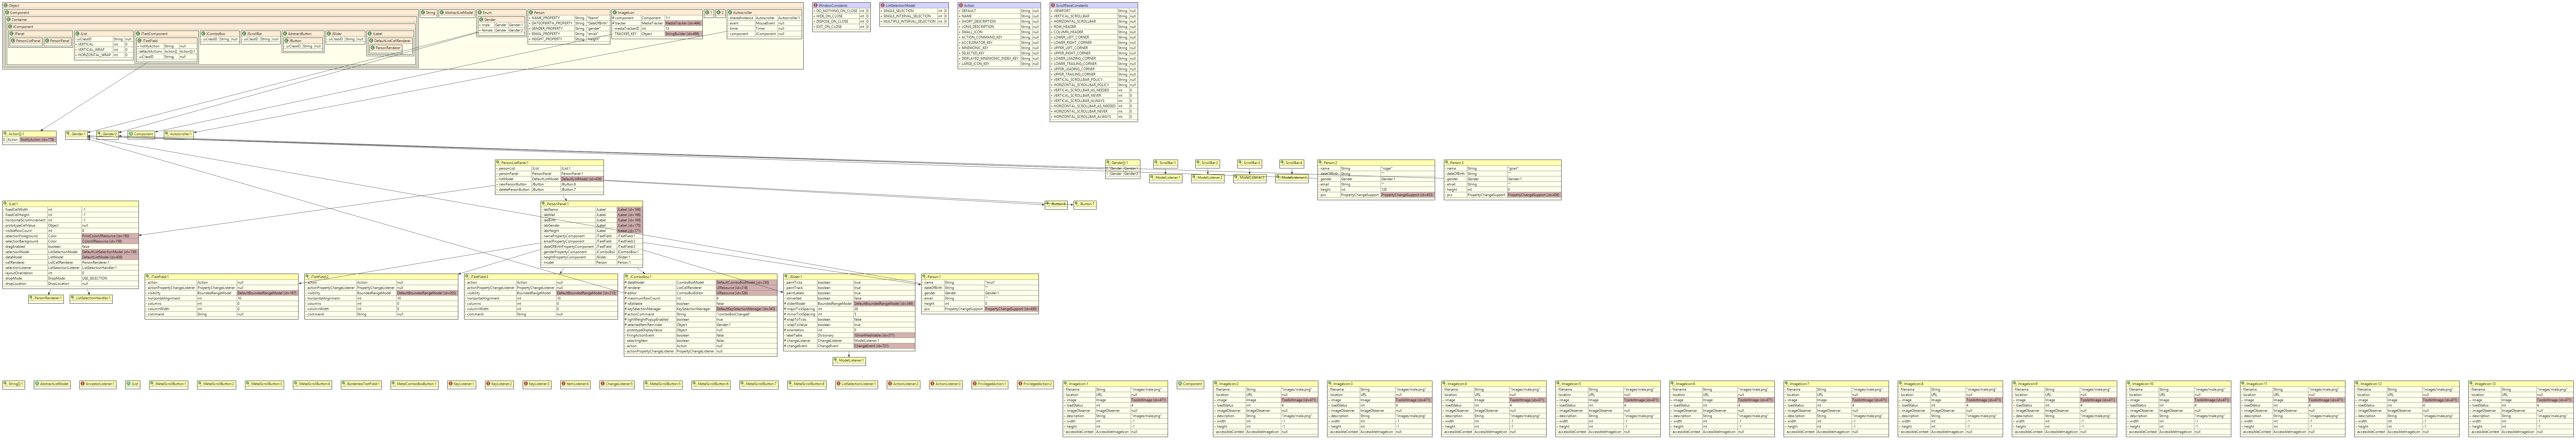
\includegraphics[width=\textwidth]{MMI-Oving4-ObjectDiagVerybig}
	\caption{Contour diagram that has grown unnecessarily large.}
	\label{fig:MMI-Oving4-ObjectDiagVerybig}
\end{figure}

Another suggestion was to make it possible to trigger the isolated view from the mentioned line of objects at the top of the sequence diagram instead of having to find the desired objects, and then scroll down to find the first event it is involved in.%finally?

\section{Conclusion}\label{conclusion}
This section will summarize the previous sections in light of the research questions proposed in the introduction.

%resultat av undersøkelse
%svar på RQ
\subsection{Research Questions}\label{conclusionRQs}


\begin{theorem}
What is the current state of the various visualization tools that are available?
\end{theorem}
There are currently several different tools that can aid a developer in his understanding of programming, ranging from the regular debuggers found in most IDEs, to code analysis and execution tracers.
Most of these focus on one or two features, instead of attempting to combine them all.
Regarding NTNUs chosen teaching environment, the amount of available tools is naturally reduced, but there is still a large portion of tools available, thanks to the plug-in support of Eclipse.
Among these, JIVE was found to be of most interest, due to its combination of features, including tracing, diagram generation, and state-jumping.
~\\

\begin{theorem}
Could any of these be integrated into the current teaching environment at NTNU, consisting of Java and Eclipse?
\end{theorem}
Both JIVE and other tools are available as Eclipse-plugins, and as such, they can easily be integrated into the courses that use Eclipse.
Unless a very platform-specific mandatory framework is used, students are of course free to choose a different IDE while following  a course, and by doing so, they will also opt out of the use of JIVE or any other tools.
But these students are not likely to be the ones that would benefit the most from such tools in the first place, as a decision to not use recommended tools usually indicates that they know what they are doing. %? ikke akkurat noe jeg har undersøkt, bør ha mer for å støtte opp om dette
~\\

\begin{theorem}
Is there room for improvement in how these tools are used, and the ease of using them?
\end{theorem}
~\\

\begin{theorem}
Would the use of such tools and any improvements actually be useful for the students?
\end{theorem}
~\\

%framtidig arbeid
\subsection{Future work}\label{conclusionFuture}




%Glossary
\printglossary
\printglossary[type=\acronymtype, style=superbold]

\newpage
~
\newpage


%Bibliography
\phantomsection
\phantomsection
\addcontentsline{toc}{chapter}{Bibliography}
\bibliographystyle{apalike}
\bibliography{Bibliography}

% appendixes. 
\appendix
\chapter{Accessing the source code}\label{appSrc}
\section{JIVE}\label{appSrcJive}
The source code of \gls{jive} can be acquired by following the installation instructions at \url{http://www.cse.buffalo.edu/jive/download.html}.
After the installation is complete, a set of jar-archive files can be found in Eclipse's plugin folder.
The plugin is divided into several archives, representing the plugin fragments.
The source code for each fragment can be found within the respective archives, and can be extracted with an appropriate program.
After extracting the code, it can be imported into Eclipse as a project.

\section{The modified version}\label{appSrcJiveMod}
The modified source code can be found at the following repository at Github: \url{https://github.com/Skabbkladden/Meister/}.
The code is located within the folders \emph{code/JIVE/}.

\end{document}
